\documentclass[aspectratio=169,xcolor=dvipsnames]{beamer}
\usetheme{SimplePlus}

% Math
\usepackage{nicefrac}

% Tipography stuff
\usepackage{booktabs} % Allows the use of \toprule, \midrule and \bottomrule in tables
\usepackage[english]{babel}
\usepackage{microtype}
\usepackage{pdfpages}
\usepackage{fontawesome5}
\usepackage{soul}
\usepackage{euler}

% Bibliography
\usepackage[giveninits,style=authoryear-comp,backend=biber]{biblatex}
\addbibresource{../fracbiblio.bib}
\newcommand\unnumbered{\setbeamertemplate{footline}{}}%\addtocounter{framenumber}{-1}
\renewcommand*{\bibfont}{\normalfont\small}

% Figures
\usepackage{tikz,pgfplots}
\usetikzlibrary{calc,arrows}
\usepackage{subfig}
\usepackage{graphicx} % Allows including images

% Links
\usepackage{hyperref}
\hypersetup{colorlinks,linkcolor=,urlcolor=MidnightBlue}

% Code
\usepackage{minted}


\author{Fabio Durastante}
\title{An introduction to fractional calculus}
\subtitle{Fundamental ideas and numerics}
\institute{Università di Pisa\\\href{mailto:fabio.durastante@unipi.it}{\faEnvelope\;fabio.durastante@unipi.it}\\\href{https://fdurastante.github.io}{\faFirefox\;fdurastante.github.io}}
\date{May, 2022}

\newcommand{\de}{{\rm d}}


\begin{document}

{\unnumbered
\begin{frame}[t,plain,noframenumbering]
\titlepage
\vspace{-4em}
\includegraphics[width=2cm]{frame.png}
\end{frame}
}

\section{The Numerical Integration of FODEs}

\begin{frame}{The Numerical Integration of FODEs}
We want to find a \textbf{numerical solution} of the differential equation written in terms of Caputo Derivatives
\begin{equation}\label{eq:fode}
\alpha > 0,\quad m = \lceil \alpha \rceil, \qquad \begin{cases}
\displaystyle {}_{C}{D_{[0,t]}^{\alpha}} \mathbf{y}(t) = f(t,\mathbf{y}(t)), & t \in [0,T],\\[0.5em]
\displaystyle \frac{d^k \mathbf{y}(0)}{d t^k}  = \mathbf{y}_0^{(k)}, & k=0,1,\ldots,m-1.
\end{cases}\tag{FODE}
\end{equation}

\begin{block}{Caputo fractional derivative~\parencite{CaputoOriginal}}
	Let $\alpha \geq 0$, and $m = \lceil \alpha \rceil$. Then, we define the operator
	\[
	{}_{C}{D_{[a,t]}^{\alpha}} y = I_{[a,t]}^{m-\alpha} \frac{d^m}{d t^m} y,
	\]
	whenever $\frac{d^m}{d t^m} y \in \mathbb{L}^1([a,b])$.
\end{block}

\end{frame}

\begin{frame}{The Numerical Integration of ODEs}
What methods do we know for ODEs?

\onslide<2->{Given a grid $\{t_j = j \tau\}_{j=1}^{N}$ and $\tau = T/N$, approximating $\mathbf{y}(t_j) \approx y^{(j)}$.}

\begin{description}
	\item<3->[Explicit methods:] Compute $y^{(j)}$ using only values $y^{(k)}$ for $k < j$
	\begin{itemize}
		\item<7-> One Step Methods: Explicit Runge-Kutta Methods (ERK)
		\item<7-> Linear Multistep Methods: Adams--Bashforth, Predictor-Corrector 
	\end{itemize}
	\item<4->[Implicit methods:] Compute $y^{(j)}$ using only values $y^{(k)}$ for $k \leq j$
	\begin{itemize}
		\item<8-> One Step Methods: Implicit Runge-Kutta Methods (IRK,DIRK,SDIRK)
		\item<8-> Linear Multistep Methods: Adams--Moulton, Backward Differentiation Formulas (BDFs), Numerical Differentiation Formulas (NDFs),\ldots
	\end{itemize}
	\item<5->[Exponential integrators:] Compute directly $y^{(N)}$ without any $y^{(j)}$ for $j < N$.
\end{description}

\onslide<9->{For both \emph{implicit} and \emph{explicit} methods we have also \alert{all-at-once} formulations, and a middle-ground represented by \alert{Implicit-Explicit} (IMEX) methods.}

\onslide<10>{Our \emph{objective} is to transport what we can for the solution of \eqref{eq:fode}.}

\end{frame}

\section{Product Integration Rules}

\begin{frame}{Product Integration Rules}
\textbf{P}roduct \textbf{I}ntegration rules were introduced in the work \parencite{YoungPI} for Integral Equations.

\onslide<2->{
From the \emph{existence results} we know that a solution to \eqref{eq:fode} is a solution to the Integral Equation
\[
y(t) = \sum_{k=0}^{m-1} \frac{t^k}{k!} y_0^{(k)} + \frac{1}{\Gamma(\alpha)} \int_{0}^{t} (t-\tau)^{\alpha-1} f(\tau,y(\tau))\,\textrm{d}\tau, \quad m = \lceil \alpha \rceil.
\]
}
\begin{itemize}
	\item<3-> Adams-Bashforth-Moulton methods are obtained by applying a \emph{quadrature formula to the integral},
	\item<4-> We can use, e.g.,
	\begin{itemize}
		\item the \textbf{fractional rectangular formula}  with nodes $\{t_j = j \tau\}_{j=1}^{n-1}$,
		\item or the \textbf{product trapezoidal quadrature formula} with nodes $\{t_j = j \tau\}_{j=1}^{n}$.
	\end{itemize}
	To obtain a \alert{predictor-corrector} method.
\end{itemize}

\end{frame}

\begin{frame}{Product Integral Rules}
The main idea behind PI rules is to approximate the integral
\[
\int_{0}^{t} (t-\tau)^{\alpha-1} f(s,y(s))\,\textrm{d}s
\] 
by approximating the vector field $f$ with suitable polynomials.\only<2->{ We build an \alert{Adams-type} method}.
\only<2->{
If we consider a grid $\{t_0,t_1,\ldots,t_N\}$ on the whole $[t_0,T]$ we can decompose the integral as
\only<1-4>{\[
y(t) = T_{m-1}(t) + \frac{1}{\Gamma(\alpha)} \sum_{j=0}^{n-1} \int_{t_j}^{t_{j+1}} (t-s)^{\alpha-1} f(\tau,y(\tau)) \,\textrm{d}\tau, \qquad t \geq t_n.
\]}\only<5->{
\[
y^{(n)} = T_{m-1}(t_n) + w_n f^{(0)} + \sum_{j=1}^{n} b_{n,j} f^{(j)},
\]
}
\begin{itemize}
	\item<3-> Replace $f$ in each sub-interval by the first–degree polynomial interpolant
	\only<3>{
	\[
	p_j(\tau) = f_{j+1} + \frac{s - t_{j+1}}{\tau_j}, \quad s \in [t_j,tj+1], \quad \tau_j = t_{j+1}-t_j, \quad f_j = f(t_j,y_j).
	\]
	}
	\item<4-> These produce the usual fractional integral that we now how to solve
	\only<4>{
	\[
	I_{n,j}^{(k)} = \frac{1}{\Gamma(\alpha)} \int_{t_j}^{t_n} (t_n - \tau)^{\alpha-1} (\tau-t_j)^k\,\textrm{d}\tau = \frac{(t_n - t_j)^{\alpha+k}}{\Gamma(\alpha+k+1)}.
	\]
	}
	\item<5> We plug everything in our expression using that:
	\[
	w_n = I_{n,0}^{(0)} - \frac{I_{n,0}^{(1)}}{\tau_0} + \frac{I_{n,1}^{(1)}}{\tau_0}, \quad b_{n_j} = \frac{ I_{n,j-1}^{(1)} - I_{n,j}^{(1)} }{\tau_{j-1}} - \frac{I_{n,j}^{(1)} - I_{n,j+1}^{(1)}}{\tau_j}, \,j\leq n-1, \quad b_{n,n} = \frac{I_{n,n-1}^{(1)}}{\tau_{n-1}}.
	\]
\end{itemize}

}
\end{frame}

\begin{frame}{Product Integral Rules - Convergence}

To discuss \textbf{convergence properties} we can piggyback on the theory of Abel's and Volterra's fractional integral equations.
\only<2->{
\begin{equation*}
\int_{0}^{t} (t-s)^{-\alpha} \only<2>{K(t,s)} y(s) \,\textrm{d}s = f(t), \quad 0 < \alpha < 1 \quad \only<2>{\text{ (Volterra's Integral Eq.)}}\only<3>{\text{ (Abel's Integral Eq.)}}
\end{equation*}
}
\only<3->{
If we \alert{discretize everything as before} we get 
\[
[ B_N \odot K_N]\mathbf{y} = \mathbf{g}, \quad B_N = \tau^{1-\alpha} [b_{i,j}], \quad K_N = [k(t_i,t_j)], \quad \odot \text{ Hadamard product}.
\]
where $\mathbf{y} = (y_0,\ldots,y_N)^T$ and $g$ contains the \textbf{initial conditions} and the \textbf{evaluations} of $f$.
\begin{block}{Convergence analysis for \parencite{CameronMcKee}}
``[Consistency of order $p$] demands that $f(t) \in \mathcal{C}^{1-\alpha}[0,T]$ which is necessary in any case for $y(t)$ to be a smooth function $\ldots$ $|y(t_i) - y_i| \leq C \tau^p$, $i=0,1,\ldots,m-1$.'' 
\end{block}
}

\end{frame}

\begin{frame}{Product Integral Rules - Convergence}
The requirements from the standard theory are \textbf{far too strong} for what we can reasonably expect from the analysis on the solution regularity we did in the last lecture.

\begin{alertblock}{Theorem~\parencite{JenniferDixon}}
Let $f$ be Lipschitz continuous with respect to the second variable and $y_n$ be the numerical approximation obtained by applying the PI trapezoidal rule on the interval $[t_0,T]$. There exist a constant $C = C_1(T-t_0)$, which does not depend on $h$, such that
\[
\| y(t_n) - y_n \| \leq C (t_n^{\alpha-1} \tau^{1+\alpha} + \tau^2), \qquad \tau = \max_{j=0,\ldots,n-1} \tau_j.
\]
\end{alertblock}

\begin{itemize}
	\item<2-> The same drop in the convergence order occurs also when higher degree polynomials are employed,
	\item<3-> When $\alpha > 1$ convergence order $2$ is obtained.
	\item[\faBrain]<4-> It doesn't make much sense to use higher-degree PI rules if $0 < \alpha < 1$.
\end{itemize}

\end{frame}

\begin{frame}{The Fractional Rectangular Formula}

Let us reduce to the case with $\alpha \in (0,1)$, $m = 1$, and a \emph{uniform mesh}.

To build it we need to \emph{approximate the integral} with the \alert{rectangule rule}
\[
\int_{0}^{t} (t-\tau)^{\alpha-1} f(\tau,y(\tau))\,\textrm{d}\tau
\]
on the grid $\{t_j = t_0 + j\tau\}_{j=1}^N$ with \emph{uniform} grid spacing $\tau$, we denote
\[
f^{(j)} = f(t_j,y^{(j)}) \text{ for } y^{(j)} \approx y(t_j),
\]
and write it as
\[
\only<1-3>{ y^{(n)} = y_0 + \frac{\tau^\alpha}{\Gamma(\alpha)} \sum_{j=0}^{\alert<3>{n-1}} b_{n-j-1}f^{(j)}, \quad b_n = \nicefrac{\displaystyle \left[(n+1)^\alpha - n^\alpha\right]}{\displaystyle \alpha}, \quad n = 1,\ldots,N.}%
\only<4>{
y^{(n)} = y_0 + \frac{\tau^\alpha}{\Gamma(\alpha)}\left( b_{0}f^{(n-1)} + \alert<4>{\sum_{j=0}^{\alert<3>{n-2}} b_{n-j-1}f^{(j)}} \right) \quad b_n = \nicefrac{\displaystyle \left[(n+1)^\alpha - n^\alpha\right]}{\displaystyle \alpha}, \quad n = 1,\ldots,N.
}
\]
\begin{itemize}
	\item<2-> This is an \alert<2>{explicit method},
	\item<3-> By construction, this is a 1-step method\ldots\onslide<4>{ but in reality \alert<4>{we need all the previous steps}!}
\end{itemize}

\end{frame}

\begin{frame}{Some observations}
\begin{itemize}
	\item[\faCode]<1-> To build the solution we have to keep in memory either the \textbf{previous solutions} or the \textbf{function evaluations},
	\item[\faCode]<2-> Using a uniform mesh the evaluation of the weights just involve the computation of real powers of integer numbers,\only<2>{ we can simplify also the fractional trapezoidal formula
	\begin{align*}
	y^{(n)} = & T_{m-1}(t_n) + \frac{\tau^\alpha}{\Gamma(\alpha+2)} \left( w_n f^{(0)} + \sum_{j=1}^{n} b_{n-j}f^{(j)} \right), \\
	w_n = &\; (\alpha + 1 - n) n^\alpha + (n-1)^{\alpha + 1}, \\ b_0 = &\; 1, \; b_n = (n-1)^{\alpha+1} - 2 n^{\alpha + 1} + (n+1)^{\alpha+1}, \; n \geq 1.
	\end{align*}
	}
	\item[\faCode]<3-> We have to compute:
	\[
	\sum_{j=0}^{n-2} b_{n-j-1}f^{(j)},
	\]
	this is a \alert{quadratic cost} with $N$, but there is a \textbf{convolution structure}, so we can expect that some FFT-based trick could come to the rescue.
	\item[\faCode]<4-> The $1$-step name is related to the number of initial values to start the computation.
\end{itemize}

\begin{block}<5>{\faLightbulb\,Predictor-Corrector algorithms}
Now that we have two schemes we can think of using them together to build a \textbf{predictor-corrector} algorithm.
\end{block}

\end{frame}

\subsection{Predictor-Corrector Scheme}

\begin{frame}{\Large Fractional Predictor-Corrector Scheme~\parencite{FRACPECE}}
We are going to write it again for $ 0 < \alpha < 1$ on a uniform mesh

\begin{enumerate}
	\item<1-> In the \emph{prediction step} we use the fractional rectangular formula
	\[
	y^{(n+1)}_P = y^{(0)} + \frac{\tau^\alpha}{\Gamma(\alpha)} \sum_{j=0}^{n} b_{j,n+1} f(t_j,y^{(j)}), \quad b_{j,n+1} = \frac{(n+1-j)^\alpha - (n-j)^\alpha}{\alpha}
	\]
	\item<2-> In the \emph{correction step} we use the fractional trapezoidal formula
	\[
	y^{(n+1)} = y^{(0)} + \frac{\tau^\alpha}{\Gamma(\alpha)} \left( \sum_{j=0}^{n} a_{j,n+1} f(t_j,y^{(j)}) + a_{n+1,n+1}f(t_{n+1},y^{(n+1)}_P) \right)
	\]
	where
	\[
	a_{j,n+1} = \begin{cases}
	\nicefrac{(n^{\alpha+1} - (n-\alpha)(n+1)^\alpha}{\alpha(\alpha+1)}, & j = 0,\\
	\nicefrac{(n-j+2)^{\alpha+1} -2(n-j+1)^{\alpha+1} + (n-j)^{\alpha+1}}{\alpha(\alpha+1)}, & j = 1,2,\ldots,n, \\
	\nicefrac{1}{\alpha(\alpha+1)}, & j = n+1.
	\end{cases}
	\]
\end{enumerate}

\end{frame}

\begin{frame}{A Fractional Predictor-Corrector Scheme}

\begin{itemize}
	\item Predictor-Corrector schemes are of interest because they represent a good \textbf{compromise} between \textbf{accuracy} and \textbf{ease of implementation}.
	\item<2> To investigate the convergence we need to look deeper into the convergence results of the two PI integral rules~\parencite{FractionalAdamsMethodsAnalysis}.
	\begin{alertblock}{Theorem~\parencite[Theorem 2.4]{FractionalAdamsMethodsAnalysis}}
	\begin{enumerate}[(a)]
	\item Let $z \in \mathcal{C}^1([0,T])$. Then\vspace{-0.5em}
	\[
	\left\lvert \int_{0}^{t_{k+1}} (t_{k+1}-t)^{\alpha-1}z(t)\,\textrm{d}t - \sum_{j=0}^{k} b_{j,k+1}z(t_j) \right\rvert \leq \frac{1}{\alpha} \|z'\|_\infty t_{k+1}^{\alpha} \tau.
	\]
	\item Let $z(t) = t^p$ for some $p \in (0,1)$. Then,\vspace{-0.5em}
	\[
	\left\lvert \int_{0}^{t_{k+1}} (t_{k+1}-t)^{\alpha-1}z(t)\,\textrm{d}t - \sum_{j=0}^{k} b_{j,k+1}z(t_j) \right\rvert \leq C_{\alpha,p}^{Re} t_{k+1}^{\alpha+p-1} \tau.
	\]
	\end{enumerate}
	\end{alertblock}
	
\end{itemize}

\end{frame}

\begin{frame}{A Fractional Predictor-Corrector Scheme}
And analogously for the product trapezoidal formula.
\begin{alertblock}{Theorem~\parencite[Theorem 2.5]{FractionalAdamsMethodsAnalysis}.}
\begin{enumerate}[(a)]
\only<1>{\item If $z \in \mathcal{C}^2([0,T])$, then there exist a constant $C_\alpha^{Tr}$ depending only on $\alpha$ such that\vspace{-0.5em}
\[
\left| \int_{0}^{t_{k+1}} (t_{k+1}-t)^{\alpha-1}z(t)\,\textrm{d}t - \sum_{j=0}^{k+1} a_{j,k+1}z(t_j) \right| \leq C_\alpha^{Tr} \|z''\|_\infty t_{k+1}^\alpha \tau^2.
\]}
\item Let $z \in \mathcal{C}^{1}([0,T])$ and assume that $z'$ fulfills a Lipschitz condition of order $\mu \in (0,1)$. Then, there exists positive constants $B_{\alpha,\mu}^{Tr}$ and $M_{z,\mu}$ such that\vspace{-0.5em}
\[
\left| \int_{0}^{t_{k+1}} (t_{k+1}-t)^{\alpha-1}z(t)\,\textrm{d}t - \sum_{j=0}^{k+1} a_{j,k+1}z(t_j) \right| \leq B_{\alpha,\mu}^{Tr} M_{z,\mu} t_{k+1}^\alpha \tau^{1+\mu}.
\] 
\only<2>{\item[(c)] Let $z(t) = t^p$ for some $p \in (0,2)$ and $\rho = \min(2,p+1)$. Then\vspace{-0.5em}
\[
\left| \int_{0}^{t_{k+1}} (t_{k+1}-t)^{\alpha-1}z(t)\,\textrm{d}t - \sum_{j=0}^{k+1} a_{j,k+1}z(t_j) \right| \leq C_{\alpha,p}^{Tr} t_{k+1}^{\alpha+p-\rho} \tau^\rho.
\]}
\end{enumerate}
\end{alertblock}
\end{frame}

\begin{frame}{A Fractional Predictor-Corrector Scheme}
Observe that for the fractional rectangular case \alert{(b)} the bound contains 
\[
t_{k+1}^{\alpha +p -1},
\]
if $\alpha+p<1$ then we get that the overall integration error becomes larger if the size
of the interval of integration becomes smaller!

Similarly for the case \alert{(c)} for the fractional trapezoidal rule
\[
\alpha < 1, \; p < 1, \; \rho = p + 1, \quad t_{k+1}^{\alpha+p-\rho},
\] 
has the same explosive behavior.

\begin{exampleblock}{Smaller intervals for harder integrals}
By making $t_{k+1}$ smaller we have two effects
\begin{enumerate}
	\item We reduce the length of the integration interval,
	\item We change the weight function in a way that makes the integral more difficult.
\end{enumerate}
\end{exampleblock}

\end{frame}

\begin{frame}{A Fractional Predictor-Corrector Scheme}

\begin{alertblock}{Lemma~\parencite[Lemma~3.1]{FractionalAdamsMethodsAnalysis}}
Assume that the solution $y$ of the initial value problem is such that
\[
\left\lvert \int_{0}^{t_{k+1}} (t_{k+1}-t)^{\alpha-1} {}_{CA}D_{[0,t]}^\alpha y(t) \, \textrm{d}t - \sum_{j=0}^{k} b_{j,k+1} {}_{CA}D_{[0,t]}^\alpha y(t)  \right\rvert \leq C_1 t_{k+1}^{\gamma_1} \tau^{\delta_1},
\]
and
\[
\left\lvert \int_{0}^{t_{k+1}} (t_{k+1}-t)^{\alpha-1} {}_{CA}D_{[0,t]}^\alpha y(t) \, \textrm{d}t - \sum_{j=0}^{k+1} a_{j,k+1} {}_{CA}D_{[0,t]}^\alpha y(t)  \right\rvert \leq C_2 t_{k+1}^{\gamma_2} \tau^{\delta_2},
\]
with some $\gamma_1,\gamma_2 \geq 0$ and $\delta_1,\delta_2 > 0$. Then, for some suitably chosen $T > 0$, we have
\[
\max_{0 \leq j \leq N} |y(t_j) - y^{(j)}| = O(\tau^q), \quad q = \min\{\delta_1+\alpha,\delta_2\}, \quad N = \lceil \nicefrac{T}{\tau} \rceil.
\]
\end{alertblock}

\end{frame}

\begin{frame}{Error bounds}
\begin{alertblock}{Theorem~\parencite[Theorem 3.2]{FractionalAdamsMethodsAnalysis}}
Let $0 < \alpha$ and assume ${}_{CA}D_{[0,t]}^\alpha y(t) \in \mathcal{C}^2([O,T])$ for some suitable $T$. Then,\vspace{-1em}
\[
\max_{0 \leq j \leq N} |y(t_j) - y^{(j)}| = \begin{cases}
O(\tau^2), & \text{ if } \alpha \geq 1,\\
O(\tau^{1+\alpha}), & \text{ if } \alpha < 1.
\end{cases}
\]
\end{alertblock}

\only<1>{\textbf{Proof.} In view of the two bounds for the Fractional Rectangular and Trapezoidal forms we can apply the previous Lemma with $\gamma_1 = \gamma_2 = \alpha > 0$, $\delta_1 = 1$, $\delta_2 = 2$. Therefore we find a bound of order $O(\tau^q)$ where
\[
q = \min \{1+\alpha,2\} = \begin{cases}
2, & \text{ if } \alpha \geq 1,\\
1+\alpha, & \text{ if } \alpha < 1.
\end{cases}
\]}\only<2-3>{
\begin{itemize}
	\item Order of convergence is a non-decreasing function of $\alpha$,
	\item Hypotheses are stated in terms of the $\alpha$th Caputo derivative of the solution,
	\only<3>{\item<3> Can we replace them by similar assumptions on $y$ itself?}
\end{itemize}
}\only<3->{
\begin{alertblock}{Theorem~ \cite[Theorem~3.3]{FractionalAdamsMethodsAnalysis}}
Let $\alpha > 1$ and assume $y \in \mathcal{C}^{1+\lceil\alpha\rceil}([0,T])$ for some suitable $T$, then\vspace{-1em}
\[
\max_{0 \leq j \leq N} |y(t_j) - y^{(j)}| = O(\tau^{1+\lceil\alpha\rceil-\alpha}).
\]
\end{alertblock}
}\only<4>{\textbf{Proof.} We need to use the characterization of Caputo's derivative
\[
{}_{CA}D_{[0,t]}^\alpha y(t) = \sum_{\ell = 0}^{m-\lceil\alpha\rceil -1}\frac{y^{(l+\lceil\alpha\rceil)}(0)}{\Gamma( \lceil\alpha\rceil - \alpha + \ell +1)} t^{\lceil\alpha\rceil-\alpha+\ell}  + g(t), \quad \begin{array}{l}
g \in \mathcal{C}^{m-\lceil\alpha\rceil}([O,T]),\\
g^{(m-\lceil\alpha\rceil)} \in \text{Lip}(\lceil\alpha\rceil-\alpha).
\end{array}
\]
}\only<5>{\textbf{Proof.} Then for $\alpha > 1$, we can apply the Lemma with $\gamma_1 = 0$, $\gamma_2 = \alpha-1 > 0$, $\delta_1 = 1$, $\delta_2 = 1 + \lceil\alpha\rceil - \alpha$ and thus $\delta_1+\alpha = 1+\alpha > 2 > \delta_2$, $\min\{\delta_1+\alpha,\delta_2\} = \delta_2$. The overall order is then $O(\tau^{\delta_2}) = O(\tau^{1+\lceil\alpha\rceil - \alpha})$.
}
\end{frame}

\begin{frame}[fragile]{An example}

\begin{example}\vspace{-1em}
\begin{equation*}
\begin{cases}
{}_{CA}D^\alpha_{[0,t]} y(t) = \frac{40320}{\Gamma(9-\alpha)} t^{8-\alpha} - 3 \frac{\Gamma(5 + \nicefrac{\alpha}{2})}{\Gamma(5-\nicefrac{\alpha}{2})} t^{4-\nicefrac{\alpha}{2}} + \frac{9}{4}\Gamma(\alpha+1) + \left( \nicefrac{3t^{\nicefrac{\alpha}{2}}}{2} - t^4 \right)^3 - y(t)^{\nicefrac{3}{2}},\\
y(0) = 0.
\end{cases}
\end{equation*}\vspace{-0.5em}
Solution: $y(t) = t^8 - 3 t^{4 + \nicefrac{\alpha}{2}} + \frac{9}{4}t^\alpha$.
\end{example}
\begin{columns}
\begin{column}{0.5\columnwidth}\definecolor{bg}{rgb}{0.95,0.95,0.95}
\begin{onlyenv}<1>
\begin{minted}[bgcolor=bg,fontsize=\small,breaklines]{matlab}
tauval = 2.^(-(1:6));
for i=1:length(hval)
 tau  = tauval(i);
 t0 = 0; T = 1;
 alpha   = 0.25;
 [T, Y] = fde_pi1_ex(alpha, f_fun, t0, T, y0, tau);
 err(i) = norm(Y - ye(T),'inf');
end
\end{minted}
\end{onlyenv}
\begin{onlyenv}<2->
\begin{tabular}{llll}
\toprule
$\alpha$ & $\tau$ & $E$ & $q$ \\
\midrule
0.25 & 5.00e-01 & 1.42e+00 & \\
& 2.50e-01 & 4.17e-01 & 1.77 \\
& 1.25e-01 & 2.13e-01 & 0.97 \\
& 6.25e-02 & 1.03e-01 & 1.05 \\
& 3.12e-02 & 5.04e-02 & 1.03 \\
& 1.56e-02 & 2.44e-02 & 1.05 \\
\bottomrule
\end{tabular}
\end{onlyenv}
\end{column}
\begin{column}{0.5\columnwidth}
\begin{onlyenv}<1-2>{
\centering

% This file was created by matlab2tikz.
%
%The latest updates can be retrieved from
%  http://www.mathworks.com/matlabcentral/fileexchange/22022-matlab2tikz-matlab2tikz
%where you can also make suggestions and rate matlab2tikz.
%
\definecolor{mycolor1}{rgb}{0.00000,0.44700,0.74100}%
\definecolor{mycolor2}{rgb}{0.85000,0.32500,0.09800}%
%
\begin{tikzpicture}

\begin{axis}[%
width=0.8\columnwidth,
height=1.45in,
at={(0.745in,0.481in)},
scale only axis,
xmin=0,
xmax=1,
xlabel style={font=\color{white!15!black}},
%xlabel={t},
ymin=0,
ymax=1.8,
ylabel style={font=\color{white!15!black}},
%ylabel={y(t)},
axis background/.style={fill=white},
legend style={at={(0.90,0.03)}, anchor=south east, legend cell align=left, align=left, draw=none, fill=none}
]
\addplot [color=mycolor1, line width=2.0pt, only marks, mark=o, mark options={solid, mycolor1}]
  table[row sep=crcr]{%
0	0\\
0.01	0.711512473537885\\
0.02	0.846135661376084\\
0.03	0.936402546792057\\
0.04	1.00622804588348\\
0.05	1.06395157957847\\
0.06	1.11355882628236\\
0.07	1.15729211131985\\
0.08	1.19654818329334\\
0.09	1.23226015451421\\
0.1	1.26508403399063\\
0.11	1.29549920953735\\
0.12	1.3238667120341\\
0.13	1.3504650018731\\
0.14	1.3755129912765\\
0.15	1.39918543093764\\
0.16	1.42162352755184\\
0.17	1.44294247263075\\
0.18	1.46323690792783\\
0.19	1.48258497505946\\
0.2	1.50105137070482\\
0.21	1.51868968886269\\
0.22	1.53554424258487\\
0.23	1.55165149947001\\
0.24	1.5670412263792\\
0.25	1.58173741238177\\
0.26	1.5957590205807\\
0.27	1.60912060651234\\
0.28	1.62183283153491\\
0.29	1.63390289287899\\
0.3	1.64533488707411\\
0.31	1.65613011977405\\
0.32	1.66628737222624\\
0.33	1.67580313251941\\
0.34	1.6846717981246\\
0.35	1.69288585499155\\
0.36	1.70043603748513\\
0.37	1.70731147267855\\
0.38	1.71349981191205\\
0.39	1.71898735204171\\
0.4	1.72375914841494\\
0.41	1.72779912129643\\
0.42	1.73109015721491\\
0.43	1.73361420649476\\
0.44	1.73535237806781\\
0.45	1.73628503252188\\
0.46	1.73639187422841\\
0.47	1.73565204329708\\
0.48	1.73404420802652\\
0.49	1.73154665845499\\
0.5	1.72813740156059\\
0.51	1.72379425861439\\
0.52	1.71849496515213\\
0.53	1.71221727399765\\
0.54	1.70493906174452\\
0.55	1.69663843907911\\
0.56	1.68729386530975\\
0.57	1.67688426744995\\
0.58	1.6653891641902\\
0.59	1.6527887950813\\
0.6	1.63906425524218\\
0.61	1.62419763589704\\
0.62	1.60817217103925\\
0.63	1.59097239051339\\
0.64	1.57258427980152\\
0.65	1.55299544679467\\
0.66	1.53219529582671\\
0.67	1.51017520924331\\
0.68	1.48692873677501\\
0.69	1.4624517929797\\
0.7	1.43674286301574\\
0.71	1.40980321700261\\
0.72	1.38163713322169\\
0.73	1.3522521304041\\
0.74	1.32165920934701\\
0.75	1.28987310409229\\
0.76	1.25691254289366\\
0.77	1.22280051918858\\
0.78	1.18756457277944\\
0.79	1.15123708141515\\
0.8	1.11385556294774\\
0.81	1.0754629882189\\
0.82	1.0361081048082\\
0.83	0.995845771746418\\
0.84	0.954737305264106\\
0.85	0.912850835604991\\
0.86	0.870261674885425\\
0.87	0.827052695922809\\
0.88	0.783314721885571\\
0.89	0.739146926532278\\
0.9	0.694657244704583\\
0.91	0.649962792613589\\
0.92	0.60519029730696\\
0.93	0.56047653451777\\
0.94	0.515968773867551\\
0.95	0.471825230114109\\
0.96	0.42821551878545\\
0.97	0.385321114105577\\
0.98	0.343335806570693\\
0.99	0.302466156840053\\
1	0.262931941713308\\
};
\addlegendentry{Numerical Approximation}

\addplot [color=mycolor2, line width=2.0pt]
  table[row sep=crcr]{%
0	0\\
0.01	0.711512456667646\\
0.02	0.846135401590434\\
0.03	0.936401508675076\\
0.04	1.00622545395592\\
0.05	1.06394641661722\\
0.06	1.11354984864932\\
0.07	1.15727785383275\\
0.08	1.19652696622605\\
0.09	1.23223008819289\\
0.1	1.26504302341549\\
0.11	1.29544495821959\\
0.12	1.3237967256148\\
0.13	1.35037659139785\\
0.14	1.37540327629225\\
0.15	1.39905134241473\\
0.16	1.42146181069809\\
0.17	1.44274968962169\\
0.18	1.46300944059051\\
0.19	1.48231902753459\\
0.2	1.50074297211395\\
0.21	1.51833469600289\\
0.22	1.53513834267313\\
0.23	1.5511902129577\\
0.24	1.56651990985671\\
0.25	1.58115126159254\\
0.26	1.59510307356365\\
0.27	1.60838974689159\\
0.28	1.62102179197548\\
0.29	1.63300625872751\\
0.3	1.6443471002035\\
0.31	1.65504548265186\\
0.32	1.66510005222637\\
0.33	1.6745071664979\\
0.34	1.6832610972806\\
0.35	1.69135421003544\\
0.36	1.6987771241369\\
0.37	1.70551885752024\\
0.38	1.71156695861958\\
0.39	1.71690762802268\\
0.4	1.72152583188042\\
0.41	1.72540540879658\\
0.42	1.72852917167004\\
0.43	1.73087900575572\\
0.44	1.73243596404175\\
0.45	1.73318036090204\\
0.46	1.73309186486972\\
0.47	1.73214959128207\\
0.48	1.73033219546997\\
0.49	1.72761796709961\\
0.5	1.72398492621998\\
0.51	1.71941092152483\\
0.52	1.71387373129965\\
0.53	1.70735116749293\\
0.54	1.69982118332455\\
0.55	1.691261984822\\
0.56	1.68165214665672\\
0.57	1.67097073263794\\
0.58	1.65919742120802\\
0.59	1.64631263627368\\
0.6	1.63229768369806\\
0.61	1.61713489377246\\
0.62	1.60080776998038\\
0.63	1.58330114436251\\
0.64	1.56460133978786\\
0.65	1.54469633943377\\
0.66	1.52357596377595\\
0.67	1.50123205538855\\
0.68	1.47765867185403\\
0.69	1.45285228708249\\
0.7	1.42681200134081\\
0.71	1.39953976029275\\
0.72	1.37104058335245\\
0.73	1.34132280165542\\
0.74	1.31039830595269\\
0.75	1.27828280473615\\
0.76	1.24499609290503\\
0.77	1.21056233128625\\
0.78	1.17501033732364\\
0.79	1.13837388725402\\
0.8	1.10069203009083\\
0.81	1.0620094137391\\
0.82	1.02237662356851\\
0.83	0.981850533774564\\
0.84	0.940494671861157\\
0.85	0.898379596580965\\
0.86	0.855583289673737\\
0.87	0.8121915617458\\
0.88	0.768298472637705\\
0.89	0.724006766630437\\
0.9	0.679428322844217\\
0.91	0.634684621187557\\
0.92	0.589907224217872\\
0.93	0.545238275278664\\
0.94	0.500831013282004\\
0.95	0.456850304508799\\
0.96	0.413473191803081\\
0.97	0.370889461540358\\
0.98	0.329302228753896\\
0.99	0.288928540806596\\
1	0.25\\
};
\addlegendentry{True Solution}

\end{axis}
\end{tikzpicture}%}
\end{onlyenv}%
\begin{onlyenv}<3>
\begin{minted}[bgcolor=bg,fontsize=\small,breaklines]{matlab}
hval = 2.^(-(1:6));
for i=1:length(hval)
 h = hval(i);
 t0 = 0; T = 1;
 [T, Y] = fde_pi12_pc(alpha, f_fun, t0, T, y0, h, [], 1);
 err(i) = norm(Y - ye(T),'inf');
end
\end{minted}
\end{onlyenv}
\begin{onlyenv}<4>
\begin{tabular}{llll}
\toprule
$\alpha$ & $\tau$ & $E$ & $q$ \\
\midrule
0.25 & 5.00e-01 & 2.75e+00 & \\
& 2.50e-01 & 1.80e+00 & 0.61 \\
& 1.25e-01 & 8.37e-01 & 1.10 \\
& 6.25e-02 & 2.45e-01 & 1.77 \\
& 3.12e-02 & 6.57e-02 & 1.90 \\
& 1.56e-02 & 2.02e-02 & 1.70 \\
\bottomrule
\end{tabular}
\end{onlyenv}
\begin{onlyenv}<5>
	\begin{tabular}{llll}
		\toprule
		$\alpha$ & $\tau$ & $E$ & $q$ \\
		\midrule
     & 1.95e-03 & 9.33e-04 & 1.42 \\
& 9.77e-04 & 3.58e-04 & 1.38 \\
& 4.88e-04 & 1.40e-04 & 1.35 \\
& 2.44e-04 & 5.56e-05 & 1.33 \\
& 1.22e-04 & 2.23e-05 & 1.32 \\
& 6.10e-05 & 9.00e-06 & 1.31 \\
		\bottomrule
	\end{tabular}
\end{onlyenv}
\end{column}
\end{columns}

\end{frame}

\begin{frame}{More than one correction step}
One can think of improving convergence by performing \textbf{more than one correction step} in the algorithm~\parencite{PredictorCorrector}.

Let us call $\mu \in \mathbb{N}$ the number of correction steps:
\[
\begin{cases}
y^{(n+1)}_{[0]} = y^{(0)} + \frac{\tau^\alpha}{\Gamma(\alpha)} \sum_{j=0}^{n} b_{j,n+1} f(t_j,y^{(j)}), & \text{Prediction step},\\
y^{(n+1)}_{[\ell]} = y^{(0)} + \frac{\tau^\alpha}{\Gamma(\alpha)} \left( \sum_{j=0}^{n} a_{j,n+1} f(t_j,y^{(j)}) + a_{n+1,n+1}f(t_{n+1},y^{(n+1)}_{[\ell-1]}) \right), & \text{Correction steps }\\
& \ell=1,\ldots,\mu.\\
y^{(n+1)} \equiv y^{(n+1)}_{[\mu]}. 
\end{cases}
\]
\begin{itemize}
	\item[\faBrain]<2-> Each iteration is expected to increase the order of convergence of a fraction $\alpha$ from order $1$ ($\mu = 0$) representing the fractional rectangular rule,
	\item[\faBrain]<3-> The standard predictor corrector method is obtained for $\mu = 1$.
\end{itemize}

\end{frame}

\begin{frame}{Convergence behavior}
The convergence behavior can be described by using repeatedly the result from \parencite[Lemma 3.1]{FractionalAdamsMethodsAnalysis} that we have used to obtain the other convergence bounds.

\begin{alertblock}{Corollary}
\[
\max_{0 \leq n \leq N} |y(t_n) - y^{(n)}| = \begin{cases}
O(\tau^{\min(1+\mu\alpha,2) }), & \text{ if } {}_{CA} D_{[t_0,t]}^\alpha y(t) \in \mathcal{C}^2([0,T]),\\
O(\tau^{\min(1+\mu\alpha,2-\alpha)}), & \text{ if } y(t) \in \mathcal{C}^2([0,T]),\\
O(\tau^{1+\alpha}), & \text{ if } f(t,y) \in \mathcal{C}^2([O,T]\times\mathbb{D}).
\end{cases}
\]
\end{alertblock}
\begin{itemize}
	\item<2-> The maximum order of convergence for ${}_{CA} D_{[t_0,t]}^\alpha y(t) \in \mathcal{C}^2([0,T])$ is obtained for $\mu = \lceil \nicefrac{1}{\alpha} \rceil$,
	\item<3-> The maximum order of convergence for $y(t) \in \mathcal{C}^2([0,T])$ is obtained for $\mu = \lceil \nicefrac{1-\alpha}{\alpha} \rceil$,
	\item<4-> In the third case with a single corrector step, and no improvement is possible.
	\item[\faLightbulb]<5> In general we could fix a maximum number of steps $\mu$ and halt the procedure when the error is under a certain tolerance.
\end{itemize}
\end{frame}

\subsection{Absolute stability}

\begin{frame}{Absolute stability}

Let us focus on the \textbf{test problem}
\[
{}_{CA} D_{[t_0,t]}^\alpha y(t) = \lambda y(t), \quad y(0) = y_0, \quad \lambda \in \mathbb{C}, \quad 0 < \alpha < 1. 
\]
In the last lecture we have seen that the solution of this problem can be expressed as
\[
y(t) = E_{\alpha}(\lambda (t - t_0)^\alpha) y_0.
\]

\begin{columns}[t]
\begin{column}{0.63\columnwidth}
\begin{block}<2->{Asymptotic behavior}
The solution $y(t)$ asymptotically vanishes as $t \rightarrow +\infty$ for 
\[
\lambda \in S^* = \{ z \in \mathbb{C}\,:\, |\arg(z) - \pi| < (1 - \nicefrac{\alpha}{2}) \pi. \}
\]
\end{block}
\only<3->{
The application of PI rule leads to a non-homogeneous difference equation\vspace{-1.5em}
\[
y^{(n)} = g^{(n)} + \sum_{j=k}^{n} c_{n-j} y^{(j)}, \quad n \geq k,
\]
where $c_n$, $g^{(n)}$ depends on $z = \tau^\alpha \lambda$.
}\end{column}
\begin{column}{0.37\columnwidth}
\centering	
	
\only<2>{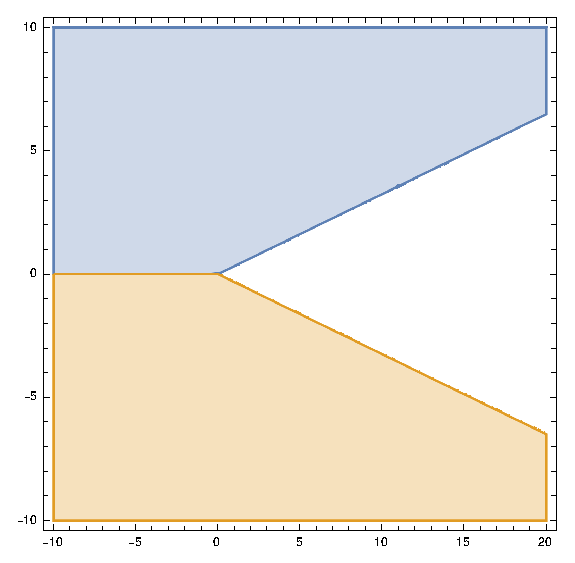
\includegraphics[width=0.75\columnwidth]{sset.eps}}
\only<3>{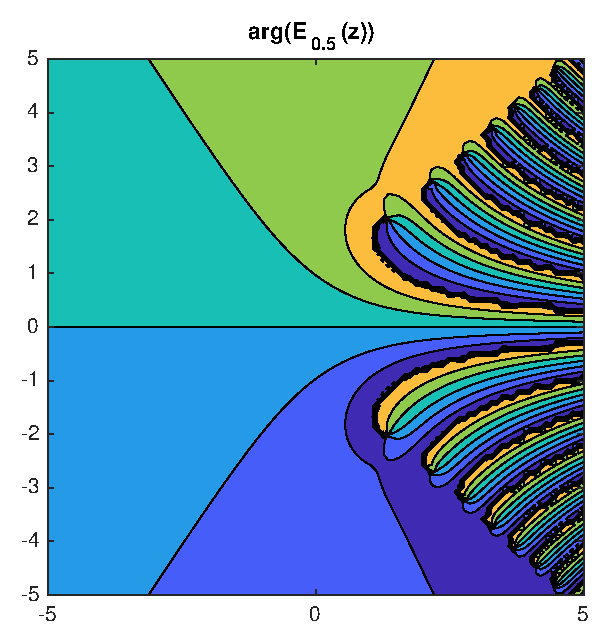
\includegraphics[width=0.75\columnwidth]{argml.eps}}
\only<4>{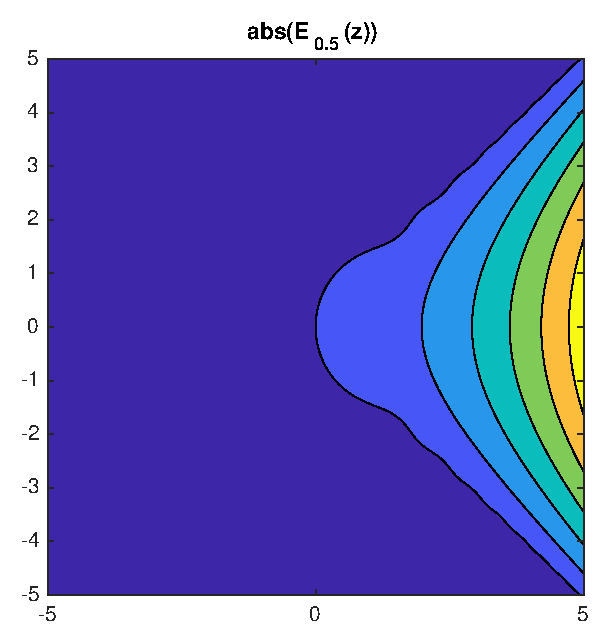
\includegraphics[width=0.75\columnwidth]{absml.eps}}
\end{column}
\end{columns}


\end{frame}

\begin{frame}{Absolute stability}
\begin{exampleblock}{Informally}
The stability region of the various PI formulas can be described as the set of all $z = \tau^\alpha \lambda$ for which the numerical solution $\{y^{(n)}\}_n$ behaves as the true solution and tends to $0$ as $n \rightarrow + \infty$.
\end{exampleblock}

\only<2->{As for the other theoretical result we are going to leverage information on the associated Volterra integral equation~\parencite{LubichConvergence}.
\begin{itemize}
	\item First we rewrite our non-homogeneous difference equation (in which we simplify the notation assuming to work with scalars) as
	\[
	\begin{cases}
	y_n =  f_n + \tau^\alpha \sum_{j=0}^{n} \omega_{n-j} g(y_j), & n \geq 0 \\
	f_n =  f(t_n) + \tau^\alpha \sum_{j=-m}^{-1} w_{n,j} g(y_j), & t_n = t_0 + n \tau, \quad t_0 = m h.
	\end{cases}
	\]
	\item Then we assume that $h^\alpha w_{n,j} g(y_j) = O( (n\tau)^{\alpha-1} \tau g(y_j) )$, i.e., $w_{n,j} = O(n^{\alpha-1})$ as $n \rightarrow + \infty$, $j=-M,\ldots,-1$.
\end{itemize}

}

\end{frame}

\begin{frame}{Absolute stability}
\begin{block}{A connection to the classical theory}
In the classical case $\alpha = 1$, if we can express the term\vspace{-0.7em}
\[
\sum_{n=0}^{+\infty} \omega_n \zeta^n = \frac{\sigma(\zeta^{-1})}{\rho(\zeta^{-1})}
\]
as a rational function, then we have found a standard Linear Multistep Method.
\end{block}

\begin{block}<2>{$A$-stable method}
A convolution quadrature $\{\omega\}_n$ for the Abel equation\vspace{-0.7em}
\[
y(t) = f(t) + \frac{1}{\Gamma(\alpha)} \int_{0}^{t} (t-s)^{\alpha-1} g[y(s)]\,\textrm{d}s, \quad t \geq 0,\;0 < \alpha \leq 1,
\]
is called $A$-stable if the solution $\{y_n\}_n$ given by the convolution quadrature satisfies\vspace{-0.7em}
\[
y_n \rightarrow 0 \text{ as } n \rightarrow + \infty \text{ whenever } \{f_n\}_n \text{ has a finite limit } \forall \tau  > 0, \; \forall\,\lambda \in S^*.
\]
\end{block}

\end{frame}

\begin{frame}{Stability region}
In general we cannot expect to have stability for every $\lambda \in S^*$, consider, e.g.
\[
{}_{CA} D_{[t_0,t]}^\alpha y(t) = - 5 y(t), \quad y(0) = 1, \quad T = 1. 
\]  
integrated with the explicit fractional rectangular rule
\begin{columns}
\begin{column}{0.33\columnwidth}
\centering

% This file was created by matlab2tikz.
%
%The latest updates can be retrieved from
%  http://www.mathworks.com/matlabcentral/fileexchange/22022-matlab2tikz-matlab2tikz
%where you can also make suggestions and rate matlab2tikz.
%
\definecolor{mycolor1}{rgb}{0.00000,0.44700,0.74100}%
\definecolor{mycolor2}{rgb}{0.85000,0.32500,0.09800}%
%
\begin{tikzpicture}

\begin{axis}[%
width=0.8\columnwidth,
height=1.25in,
at={(0.758in,0.481in)},
scale only axis,
xmin=0,
xmax=1,
xlabel style={font=\color{white!15!black}},
%xlabel={t},
ymin=-20,
ymax=30,
ylabel style={font=\color{white!15!black}},
%ylabel={y(t)},
axis background/.style={fill=white},
legend style={legend cell align=left, align=left, draw=white!15!black}
]
\addplot [color=mycolor1, line width=2.0pt, only marks, mark=o, mark options={solid, mycolor1}]
  table[row sep=crcr]{%
0	1\\
0.1	-0.784124116152771\\
0.2	1.65996633981775\\
0.3	-1.94917275995581\\
0.4	3.21742871214999\\
0.5	-4.28745985055969\\
0.6	6.53288133991967\\
0.7	-9.13038883698865\\
0.8	13.4925614630154\\
0.9	-19.2245778843926\\
1	28.0550017583399\\
};
%\addlegendentry{Numerical Approximation}

\addplot [color=mycolor2, line width=2.0pt]
  table[row sep=crcr]{%
0	1\\
0.1	0.308793556708284\\
0.2	0.232326294376465\\
0.3	0.194384767555019\\
0.4	0.170577718325973\\
0.5	0.153838609950013\\
0.6	0.141236687931621\\
0.7	0.131304435585141\\
0.8	0.123213940087892\\
0.9	0.116457644686649\\
1	0.110704637733069\\
};
%\addlegendentry{True Solution}

\end{axis}
\end{tikzpicture}%

$h = 10^{-1}$\vfill
\end{column}
\begin{column}{0.33\columnwidth}
\centering

% This file was created by matlab2tikz.
%
%The latest updates can be retrieved from
%  http://www.mathworks.com/matlabcentral/fileexchange/22022-matlab2tikz-matlab2tikz
%where you can also make suggestions and rate matlab2tikz.
%
\definecolor{mycolor1}{rgb}{0.00000,0.44700,0.74100}%
\definecolor{mycolor2}{rgb}{0.85000,0.32500,0.09800}%
%
\begin{tikzpicture}

\begin{axis}[%
width=0.8\columnwidth,
height=1.25in,
at={(0.758in,0.481in)},
scale only axis,
xmin=0,
xmax=1,
xlabel style={font=\color{white!15!black}},
%xlabel={t},
ymin=0.1,
ymax=1,
ylabel style={font=\color{white!15!black}},
%ylabel={y(t)},
axis background/.style={fill=white},
legend style={legend cell align=left, align=left, draw=white!15!black}
]
\addplot [color=mycolor1, line width=2.0pt, only marks, mark=o, mark options={solid, mycolor1}]
  table[row sep=crcr]{%
0	1\\
0.01	0.435810416452244\\
0.02	0.520425325380925\\
0.03	0.425214284042309\\
0.04	0.409153876640326\\
0.05	0.377395931729297\\
0.06	0.35808080580884\\
0.07	0.339609189688472\\
0.08	0.324567877155222\\
0.09	0.311217349716659\\
0.1	0.299540372748172\\
0.11	0.289108517016612\\
0.12	0.279743251326986\\
0.13	0.271258675265005\\
0.14	0.263525830169038\\
0.15	0.256436285320742\\
0.16	0.249904282525226\\
0.17	0.243858911388732\\
0.18	0.238241636197337\\
0.19	0.233003383236946\\
0.2	0.228102725532727\\
0.21	0.223504374051045\\
0.22	0.21917805543224\\
0.23	0.215097620228538\\
0.24	0.211240342988757\\
0.25	0.207586361757516\\
0.26	0.204118226955392\\
0.27	0.200820534538475\\
0.28	0.197679625560545\\
0.29	0.194683338247017\\
0.3	0.191820802042401\\
0.31	0.189082265438174\\
0.32	0.18645895119694\\
0.33	0.183942933943016\\
0.34	0.18152703613078\\
0.35	0.179204739203474\\
0.36	0.17697010737859\\
0.37	0.174817721984343\\
0.38	0.172742624656887\\
0.39	0.170740268013915\\
0.4	0.168806472664735\\
0.41	0.166937389613457\\
0.42	0.165129467270854\\
0.43	0.163379422419597\\
0.44	0.161684214583057\\
0.45	0.160041023334554\\
0.46	0.158447228155269\\
0.47	0.156900390508272\\
0.48	0.155398237845327\\
0.49	0.153938649304203\\
0.5	0.152519642888712\\
0.51	0.151139363952683\\
0.52	0.149796074833558\\
0.53	0.148488145502025\\
0.54	0.147214045111797\\
0.55	0.145972334348578\\
0.56	0.144761658490225\\
0.57	0.143580741101063\\
0.58	0.142428378292837\\
0.59	0.14130343349295\\
0.6	0.140204832667708\\
0.61	0.13913155995445\\
0.62	0.138082653661702\\
0.63	0.137057202601242\\
0.64	0.136054342719878\\
0.65	0.135073254002415\\
0.66	0.13411315762029\\
0.67	0.133173313303157\\
0.68	0.132253016913027\\
0.69	0.131351598202793\\
0.7	0.130468418742711\\
0.71	0.129602870000188\\
0.72	0.128754371559597\\
0.73	0.127922369470211\\
0.74	0.127106334711476\\
0.75	0.126305761765871\\
0.76	0.125520167290552\\
0.77	0.124749088879786\\
0.78	0.12399208391091\\
0.79	0.123248728467233\\
0.8	0.12251861633187\\
0.81	0.121801358047067\\
0.82	0.121096580033992\\
0.83	0.120403923768495\\
0.84	0.119723045008618\\
0.85	0.119053613070107\\
0.86	0.118395310146391\\
0.87	0.117747830669858\\
0.88	0.117110880711489\\
0.89	0.116484177416148\\
0.9	0.115867448471046\\
0.91	0.11526043160512\\
0.92	0.114662874117177\\
0.93	0.114074532430924\\
0.94	0.113495171675037\\
0.95	0.112924565286658\\
0.96	0.112362494636755\\
0.97	0.11180874867598\\
0.98	0.11126312359965\\
0.99	0.110725422530692\\
1	0.110195455219396\\
};
%\addlegendentry{Numerical Approximation}

\addplot [color=mycolor2, line width=2.0pt]
  table[row sep=crcr]{%
0	1\\
0.01	0.615690344192926\\
0.02	0.523156583730247\\
0.03	0.467161276850258\\
0.04	0.427583576155807\\
0.05	0.397362624480641\\
0.06	0.373165674278016\\
0.07	0.353153228388942\\
0.08	0.336204002446341\\
0.09	0.321585416454318\\
0.1	0.308793556708284\\
0.11	0.297467697391153\\
0.12	0.287341249533456\\
0.13	0.27821198311742\\
0.14	0.269923108221304\\
0.15	0.26235079494099\\
0.16	0.255395676310506\\
0.17	0.248976904778985\\
0.18	0.243027896711125\\
0.19	0.237493222760631\\
0.2	0.232326294376465\\
0.21	0.227487614918745\\
0.22	0.222943438573149\\
0.23	0.218664728666687\\
0.24	0.214626339069821\\
0.25	0.210806364061144\\
0.26	0.207185616965641\\
0.27	0.203747208331724\\
0.28	0.200476201841176\\
0.29	0.197359331498842\\
0.3	0.194384767555019\\
0.31	0.191541921497594\\
0.32	0.188821282603938\\
0.33	0.18621428016587\\
0.34	0.183713166736723\\
0.35	0.181310918698449\\
0.36	0.17900115118139\\
0.37	0.176778044942644\\
0.38	0.174636283259535\\
0.39	0.172570997251279\\
0.4	0.170577718325973\\
0.41	0.168652336677644\\
0.42	0.166791064941571\\
0.43	0.164990406264784\\
0.44	0.163247126169801\\
0.45	0.161558227688845\\
0.46	0.15992092932739\\
0.47	0.158332645483292\\
0.48	0.156790969003743\\
0.49	0.155293655608894\\
0.5	0.153838609950013\\
0.51	0.152423873102776\\
0.52	0.151047611323943\\
0.53	0.149708105922947\\
0.54	0.148403744119789\\
0.55	0.147133010777457\\
0.56	0.145894480911485\\
0.57	0.144686812891607\\
0.58	0.143508742261014\\
0.59	0.142359076107878\\
0.6	0.141236687931621\\
0.61	0.14014051295327\\
0.62	0.139069543825104\\
0.63	0.138022826699964\\
0.64	0.136999457625061\\
0.65	0.135998579229042\\
0.66	0.135019377674489\\
0.67	0.134061079851043\\
0.68	0.133122950786979\\
0.69	0.13220429125938\\
0.7	0.131304435585141\\
0.71	0.130422749576806\\
0.72	0.129558628648894\\
0.73	0.128711496061758\\
0.74	0.127880801291324\\
0.75	0.127066018514161\\
0.76	0.126266645198345\\
0.77	0.125482200791495\\
0.78	0.124712225498141\\
0.79	0.123956279139313\\
0.8	0.123213940087892\\
0.81	0.122484804273841\\
0.82	0.121768484253939\\
0.83	0.121064608341141\\
0.84	0.120372819789089\\
0.85	0.119692776027686\\
0.86	0.119024147945991\\
0.87	0.118366619219015\\
0.88	0.117719885675268\\
0.89	0.117083654702165\\
0.9	0.116457644686649\\
0.91	0.115841584488587\\
0.92	0.115235212944687\\
0.93	0.114638278400862\\
0.94	0.114050538271148\\
0.95	0.113471758621388\\
0.96	0.112901713776073\\
0.97	0.112340185946817\\
0.98	0.111786964881081\\
0.99	0.111241847529851\\
1	0.110704637733069\\
};
%\addlegendentry{True Solution}

\end{axis}
\end{tikzpicture}%

$h = 10^{-2}$\vfill
\end{column}
\begin{column}{0.33\columnwidth}
\centering

% This file was created by matlab2tikz.
%
%The latest updates can be retrieved from
%  http://www.mathworks.com/matlabcentral/fileexchange/22022-matlab2tikz-matlab2tikz
%where you can also make suggestions and rate matlab2tikz.
%
\definecolor{mycolor1}{rgb}{0.00000,0.44700,0.74100}%
\definecolor{mycolor2}{rgb}{0.85000,0.32500,0.09800}%
%
\begin{tikzpicture}

\begin{axis}[%
width=0.8\columnwidth,
height=1.25in,
at={(0.772in,0.481in)},
scale only axis,
xmin=0,
xmax=1,
xlabel style={font=\color{white!15!black}},
%xlabel={t},
ymin=0.1,
ymax=1,
ylabel style={font=\color{white!15!black}},
%ylabel={y(t)},
axis background/.style={fill=white},
legend style={legend cell align=left, align=left, draw=white!15!black}
]
\addplot [color=mycolor1, line width=2.0pt, only marks, mark=o, mark options={solid, mycolor1}]
  table[row sep=crcr]{%
0	1\\
0.001	0.821587588384723\\
0.002	0.779517736416363\\
0.003	0.743502237935276\\
0.004	0.715348459420956\\
0.005	0.691830266706237\\
0.006	0.67159744484362\\
0.007	0.653813275637237\\
0.008	0.63793529039951\\
0.009	0.623588256957663\\
0.01	0.610500804534633\\
0.011	0.598469670935461\\
0.012	0.587338284482556\\
0.013	0.576983241691229\\
0.014	0.567305403441403\\
0.015	0.558223823824714\\
0.016	0.549671486828914\\
0.017	0.541592236272532\\
0.018	0.533938516404654\\
0.019	0.526669677221584\\
0.02	0.519750681900204\\
0.021	0.513151106172541\\
0.022	0.506844353343309\\
0.023	0.50080703107505\\
0.024	0.495018451228725\\
0.025	0.489460224501111\\
0.026	0.484115928933861\\
0.027	0.478970836596072\\
0.028	0.474011686522022\\
0.029	0.469226494755623\\
0.03	0.464604394407865\\
0.031	0.460135500175023\\
0.032	0.455810792934023\\
0.033	0.451622020925897\\
0.034	0.447561614729255\\
0.035	0.443622613763997\\
0.036	0.439798602488035\\
0.037	0.436083654784174\\
0.038	0.432472285300489\\
0.039	0.42895940672106\\
0.04	0.425540292116107\\
0.041	0.422210541660337\\
0.042	0.418966053122313\\
0.043	0.415802995621187\\
0.044	0.412717786224228\\
0.045	0.409707069022413\\
0.046	0.406767696374481\\
0.047	0.403896712054218\\
0.048	0.401091336072963\\
0.049	0.398348950980714\\
0.05	0.395667089475673\\
0.051	0.393043423174599\\
0.052	0.390475752415455\\
0.053	0.387961996980196\\
0.054	0.385500187639549\\
0.055	0.383088458433677\\
0.056	0.380725039612983\\
0.057	0.378408251172301\\
0.058	0.37613649691945\\
0.059	0.373908259025926\\
0.06	0.371722093013354\\
0.061	0.369576623134451\\
0.062	0.367470538111787\\
0.063	0.365402587201514\\
0.064	0.363371576552732\\
0.065	0.361376365836225\\
0.066	0.359415865118934\\
0.067	0.357489031962991\\
0.068	0.355594868730183\\
0.069	0.353732420074638\\
0.07	0.351900770608145\\
0.071	0.35009904272405\\
0.072	0.348326394566958\\
0.073	0.346582018136662\\
0.074	0.344865137515808\\
0.075	0.343175007211701\\
0.076	0.341510910603566\\
0.077	0.339872158487301\\
0.078	0.338258087710482\\
0.079	0.336668059890977\\
0.08	0.335101460213098\\
0.081	0.333557696295752\\
0.082	0.332036197127455\\
0.083	0.330536412063555\\
0.084	0.329057809881342\\
0.085	0.327599877889092\\
0.086	0.32616212108539\\
0.087	0.324744061365376\\
0.088	0.3233452367708\\
0.089	0.321965200781027\\
0.09	0.320603521642343\\
0.091	0.3192597817331\\
0.092	0.317933576962437\\
0.093	0.316624516200475\\
0.094	0.315332220738017\\
0.095	0.314056323773967\\
0.096	0.312796469928755\\
0.097	0.311552314782224\\
0.098	0.310323524434512\\
0.099	0.309109775088572\\
0.1	0.307910752653068\\
0.101	0.306726152364473\\
0.102	0.305555678427252\\
0.103	0.304399043671128\\
0.104	0.303255969224442\\
0.105	0.302126184202739\\
0.106	0.301009425411711\\
0.107	0.299905437063737\\
0.108	0.298813970507265\\
0.109	0.297734783968348\\
0.11	0.296667642303704\\
0.111	0.295612316764661\\
0.112	0.294568584771446\\
0.113	0.293536229697267\\
0.114	0.292515040661683\\
0.115	0.291504812332793\\
0.116	0.2905053447378\\
0.117	0.28951644308152\\
0.118	0.288537917572452\\
0.119	0.287569583256025\\
0.12	0.286611259854684\\
0.121	0.285662771614466\\
0.122	0.284723947157769\\
0.123	0.283794619342008\\
0.124	0.282874625123879\\
0.125	0.281963805428978\\
0.126	0.281062005026511\\
0.127	0.280169072408863\\
0.128	0.27928485967581\\
0.129	0.278409222423153\\
0.13	0.277542019635576\\
0.131	0.276683113583544\\
0.132	0.275832369724051\\
0.133	0.27498965660505\\
0.134	0.274154845773412\\
0.135	0.273327811686248\\
0.136	0.272508431625453\\
0.137	0.271696585615335\\
0.138	0.270892156343194\\
0.139	0.270095029082723\\
0.14	0.269305091620128\\
0.141	0.268522234182822\\
0.142	0.267746349370626\\
0.143	0.266977332089334\\
0.144	0.266215079486572\\
0.145	0.26545949088985\\
0.146	0.264710467746712\\
0.147	0.263967913566907\\
0.148	0.263231733866498\\
0.149	0.262501836113827\\
0.15	0.261778129677276\\
0.151	0.261060525774736\\
0.152	0.260348937424734\\
0.153	0.259643279399135\\
0.154	0.258943468177389\\
0.155	0.258249421902221\\
0.156	0.25756106033675\\
0.157	0.256878304822962\\
0.158	0.25620107824148\\
0.159	0.255529304972611\\
0.16	0.254862910858585\\
0.161	0.254201823166976\\
0.162	0.253545970555234\\
0.163	0.252895283036317\\
0.164	0.252249691945347\\
0.165	0.25160912990729\\
0.166	0.250973530805597\\
0.167	0.250342829751781\\
0.168	0.249716963055901\\
0.169	0.249095868197914\\
0.17	0.24847948379987\\
0.171	0.247867749598914\\
0.172	0.247260606421076\\
0.173	0.246657996155813\\
0.174	0.246059861731288\\
0.175	0.245466147090347\\
0.176	0.244876797167182\\
0.177	0.244291757864654\\
0.178	0.243710976032248\\
0.179	0.243134399444649\\
0.18	0.242561976780908\\
0.181	0.24199365760419\\
0.182	0.241429392342072\\
0.183	0.240869132267386\\
0.184	0.240312829479577\\
0.185	0.239760436886569\\
0.186	0.239211908187121\\
0.187	0.238667197853651\\
0.188	0.23812626111552\\
0.189	0.237589053942761\\
0.19	0.237055533030234\\
0.191	0.236525655782198\\
0.192	0.235999380297288\\
0.193	0.235476665353878\\
0.194	0.234957470395828\\
0.195	0.234441755518593\\
0.196	0.233929481455691\\
0.197	0.233420609565513\\
0.198	0.232915101818469\\
0.199	0.23241292078446\\
0.2	0.231914029620661\\
0.201	0.231418392059613\\
0.202	0.230925972397609\\
0.203	0.230436735483367\\
0.204	0.229950646706985\\
0.205	0.229467671989166\\
0.206	0.228987777770702\\
0.207	0.228510931002222\\
0.208	0.228037099134178\\
0.209	0.227566250107078\\
0.21	0.227098352341956\\
0.211	0.226633374731062\\
0.212	0.226171286628777\\
0.213	0.225712057842746\\
0.214	0.225255658625211\\
0.215	0.224802059664558\\
0.216	0.224351232077049\\
0.217	0.223903147398762\\
0.218	0.2234577775777\\
0.219	0.223015094966094\\
0.22	0.222575072312878\\
0.221	0.222137682756334\\
0.222	0.22170289981691\\
0.223	0.221270697390196\\
0.224	0.220841049740054\\
0.225	0.220413931491917\\
0.226	0.219989317626218\\
0.227	0.219567183471983\\
0.228	0.219147504700555\\
0.229	0.218730257319459\\
0.23	0.218315417666404\\
0.231	0.217902962403415\\
0.232	0.217492868511092\\
0.233	0.217085113282993\\
0.234	0.216679674320141\\
0.235	0.216276529525652\\
0.236	0.215875657099465\\
0.237	0.215477035533199\\
0.238	0.215080643605117\\
0.239	0.214686460375187\\
0.24	0.214294465180258\\
0.241	0.21390463762933\\
0.242	0.213516957598932\\
0.243	0.213131405228583\\
0.244	0.212747960916361\\
0.245	0.212366605314553\\
0.246	0.211987319325402\\
0.247	0.211610084096936\\
0.248	0.211234881018888\\
0.249	0.21086169171869\\
0.25	0.21049049805756\\
0.251	0.210121282126659\\
0.252	0.209754026243327\\
0.253	0.209388712947401\\
0.254	0.209025324997594\\
0.255	0.20866384536796\\
0.256	0.20830425724442\\
0.257	0.20794654402136\\
0.258	0.207590689298294\\
0.259	0.207236676876594\\
0.26	0.206884490756285\\
0.261	0.2065341151329\\
0.262	0.206185534394397\\
0.263	0.205838733118135\\
0.264	0.20549369606791\\
0.265	0.205150408191047\\
0.266	0.204808854615543\\
0.267	0.204469020647276\\
0.268	0.204130891767252\\
0.269	0.20379445362892\\
0.27	0.20345969205552\\
0.271	0.203126593037497\\
0.272	0.202795142729956\\
0.273	0.202465327450159\\
0.274	0.202137133675082\\
0.275	0.201810548039006\\
0.276	0.201485557331158\\
0.277	0.20116214849339\\
0.278	0.200840308617907\\
0.279	0.200520024945034\\
0.28	0.200201284861022\\
0.281	0.199884075895893\\
0.282	0.199568385721333\\
0.283	0.199254202148606\\
0.284	0.198941513126526\\
0.285	0.198630306739443\\
0.286	0.198320571205289\\
0.287	0.198012294873637\\
0.288	0.197705466223807\\
0.289	0.197400073863004\\
0.29	0.197096106524483\\
0.291	0.196793553065756\\
0.292	0.196492402466815\\
0.293	0.196192643828407\\
0.294	0.195894266370317\\
0.295	0.195597259429701\\
0.296	0.195301612459426\\
0.297	0.195007315026465\\
0.298	0.19471435681029\\
0.299	0.194422727601319\\
0.3	0.194132417299371\\
0.301	0.193843415912161\\
0.302	0.193555713553804\\
0.303	0.193269300443361\\
0.304	0.192984166903403\\
0.305	0.192700303358593\\
0.306	0.192417700334301\\
0.307	0.192136348455236\\
0.308	0.191856238444106\\
0.309	0.191577361120296\\
0.31	0.191299707398566\\
0.311	0.191023268287776\\
0.312	0.190748034889629\\
0.313	0.190473998397435\\
0.314	0.190201150094895\\
0.315	0.189929481354904\\
0.316	0.189658983638374\\
0.317	0.189389648493078\\
0.318	0.18912146755251\\
0.319	0.188854432534761\\
0.32	0.188588535241421\\
0.321	0.188323767556494\\
0.322	0.188060121445322\\
0.323	0.187797588953545\\
0.324	0.187536162206057\\
0.325	0.187275833405993\\
0.326	0.187016594833727\\
0.327	0.186758438845884\\
0.328	0.186501357874368\\
0.329	0.18624534442541\\
0.33	0.185990391078623\\
0.331	0.185736490486077\\
0.332	0.18548363537139\\
0.333	0.185231818528825\\
0.334	0.184981032822407\\
0.335	0.184731271185057\\
0.336	0.184482526617728\\
0.337	0.184234792188566\\
0.338	0.183988061032076\\
0.339	0.183742326348302\\
0.34	0.183497581402024\\
0.341	0.183253819521961\\
0.342	0.18301103409999\\
0.343	0.182769218590375\\
0.344	0.182528366509007\\
0.345	0.182288471432658\\
0.346	0.182049526998241\\
0.347	0.181811526902088\\
0.348	0.181574464899234\\
0.349	0.181338334802709\\
0.35	0.18110313048285\\
0.351	0.18086884586661\\
0.352	0.180635474936891\\
0.353	0.180403011731873\\
0.354	0.180171450344366\\
0.355	0.179940784921158\\
0.356	0.179711009662388\\
0.357	0.179482118820909\\
0.358	0.17925410670168\\
0.359	0.179026967661152\\
0.36	0.178800696106667\\
0.361	0.178575286495873\\
0.362	0.178350733336134\\
0.363	0.178127031183959\\
0.364	0.177904174644433\\
0.365	0.177682158370663\\
0.366	0.177460977063221\\
0.367	0.177240625469605\\
0.368	0.177021098383704\\
0.369	0.176802390645268\\
0.37	0.176584497139387\\
0.371	0.17636741279598\\
0.372	0.17615113258929\\
0.373	0.175935651537377\\
0.374	0.175720964701637\\
0.375	0.175507067186305\\
0.376	0.175293954137987\\
0.377	0.175081620745177\\
0.378	0.174870062237802\\
0.379	0.174659273886752\\
0.38	0.174449251003434\\
0.381	0.174239988939321\\
0.382	0.174031483085514\\
0.383	0.173823728872303\\
0.384	0.17361672176874\\
0.385	0.173410457282217\\
0.386	0.173204930958044\\
0.387	0.173000138379038\\
0.388	0.172796075165121\\
0.389	0.17259273697291\\
0.39	0.172390119495328\\
0.391	0.172188218461208\\
0.392	0.171987029634914\\
0.393	0.171786548815951\\
0.394	0.171586771838598\\
0.395	0.171387694571531\\
0.396	0.171189312917462\\
0.397	0.170991622812774\\
0.398	0.170794620227166\\
0.399	0.170598301163301\\
0.4	0.17040266165646\\
0.401	0.170207697774196\\
0.402	0.170013405616001\\
0.403	0.169819781312964\\
0.404	0.16962682102745\\
0.405	0.169434520952766\\
0.406	0.169242877312847\\
0.407	0.169051886361935\\
0.408	0.168861544384264\\
0.409	0.168671847693753\\
0.41	0.168482792633703\\
0.411	0.168294375576489\\
0.412	0.168106592923269\\
0.413	0.167919441103683\\
0.414	0.167732916575571\\
0.415	0.167547015824675\\
0.416	0.16736173536437\\
0.417	0.16717707173537\\
0.418	0.166993021505464\\
0.419	0.166809581269231\\
0.42	0.166626747647783\\
0.421	0.16644451728849\\
0.422	0.16626288686472\\
0.423	0.166081853075582\\
0.424	0.165901412645663\\
0.425	0.165721562324782\\
0.426	0.165542298887735\\
0.427	0.165363619134048\\
0.428	0.165185519887736\\
0.429	0.16500799799706\\
0.43	0.164831050334285\\
0.431	0.16465467379545\\
0.432	0.164478865300134\\
0.433	0.164303621791222\\
0.434	0.164128940234685\\
0.435	0.163954817619349\\
0.436	0.163781250956674\\
0.437	0.163608237280544\\
0.438	0.163435773647034\\
0.439	0.163263857134211\\
0.44	0.163092484841917\\
0.441	0.162921653891555\\
0.442	0.162751361425892\\
0.443	0.16258160460885\\
0.444	0.162412380625301\\
0.445	0.162243686680873\\
0.446	0.162075520001754\\
0.447	0.161907877834489\\
0.448	0.161740757445797\\
0.449	0.161574156122375\\
0.45	0.161408071170712\\
0.451	0.161242499916903\\
0.452	0.161077439706464\\
0.453	0.160912887904153\\
0.454	0.160748841893786\\
0.455	0.160585299078064\\
0.456	0.160422256878397\\
0.457	0.160259712734726\\
0.458	0.160097664105357\\
0.459	0.159936108466788\\
0.46	0.159775043313543\\
0.461	0.159614466158006\\
0.462	0.159454374530256\\
0.463	0.159294765977906\\
0.464	0.159135638065942\\
0.465	0.158976988376564\\
0.466	0.158818814509033\\
0.467	0.15866111407951\\
0.468	0.158503884720909\\
0.469	0.158347124082741\\
0.47	0.158190829830963\\
0.471	0.158034999647839\\
0.472	0.157879631231781\\
0.473	0.157724722297211\\
0.474	0.157570270574419\\
0.475	0.157416273809416\\
0.476	0.1572627297638\\
0.477	0.157109636214608\\
0.478	0.156956990954192\\
0.479	0.156804791790069\\
0.48	0.156653036544797\\
0.481	0.156501723055841\\
0.482	0.156350849175434\\
0.483	0.156200412770458\\
0.484	0.156050411722307\\
0.485	0.155900843926763\\
0.486	0.155751707293872\\
0.487	0.155602999747815\\
0.488	0.15545471922679\\
0.489	0.155306863682886\\
0.49	0.155159431081967\\
0.491	0.155012419403544\\
0.492	0.154865826640671\\
0.493	0.154719650799815\\
0.494	0.154573889900746\\
0.495	0.154428541976425\\
0.496	0.154283605072886\\
0.497	0.154139077249128\\
0.498	0.153994956577004\\
0.499	0.153851241141107\\
0.5	0.153707929038668\\
0.501	0.153565018379443\\
0.502	0.153422507285612\\
0.503	0.15328039389167\\
0.504	0.153138676344323\\
0.505	0.15299735280239\\
0.506	0.152856421436695\\
0.507	0.152715880429968\\
0.508	0.152575727976749\\
0.509	0.152435962283283\\
0.51	0.152296581567429\\
0.511	0.152157584058557\\
0.512	0.152018967997455\\
0.513	0.151880731636237\\
0.514	0.151742873238245\\
0.515	0.151605391077956\\
0.516	0.151468283440893\\
0.517	0.151331548623534\\
0.518	0.151195184933218\\
0.519	0.151059190688061\\
0.52	0.150923564216864\\
0.521	0.150788303859025\\
0.522	0.150653407964457\\
0.523	0.150518874893499\\
0.524	0.150384703016831\\
0.525	0.150250890715391\\
0.526	0.150117436380291\\
0.527	0.149984338412737\\
0.528	0.149851595223945\\
0.529	0.149719205235062\\
0.53	0.149587166877084\\
0.531	0.149455478590777\\
0.532	0.149324138826607\\
0.533	0.149193146044645\\
0.534	0.149062498714509\\
0.535	0.148932195315276\\
0.536	0.148802234335409\\
0.537	0.148672614272687\\
0.538	0.148543333634126\\
0.539	0.148414390935906\\
0.54	0.148285784703304\\
0.541	0.148157513470616\\
0.542	0.148029575781089\\
0.543	0.14790197018685\\
0.544	0.147774695248837\\
0.545	0.14764774953673\\
0.546	0.147521131628879\\
0.547	0.147394840112245\\
0.548	0.147268873582324\\
0.549	0.147143230643082\\
0.55	0.147017909906895\\
0.551	0.146892909994479\\
0.552	0.146768229534826\\
0.553	0.146643867165141\\
0.554	0.146519821530778\\
0.555	0.146396091285178\\
0.556	0.146272675089808\\
0.557	0.146149571614094\\
0.558	0.146026779535369\\
0.559	0.145904297538803\\
0.56	0.145782124317351\\
0.561	0.14566025857169\\
0.562	0.145538699010158\\
0.563	0.145417444348702\\
0.564	0.145296493310818\\
0.565	0.145175844627486\\
0.566	0.145055497037129\\
0.567	0.144935449285542\\
0.568	0.144815700125847\\
0.569	0.144696248318429\\
0.57	0.144577092630891\\
0.571	0.144458231837993\\
0.572	0.144339664721601\\
0.573	0.144221390070631\\
0.574	0.144103406681005\\
0.575	0.143985713355586\\
0.576	0.143868308904139\\
0.577	0.143751192143273\\
0.578	0.143634361896389\\
0.579	0.143517816993635\\
0.58	0.143401556271854\\
0.581	0.143285578574533\\
0.582	0.143169882751754\\
0.583	0.143054467660152\\
0.584	0.142939332162859\\
0.585	0.142824475129458\\
0.586	0.142709895435939\\
0.587	0.142595591964653\\
0.588	0.14248156360426\\
0.589	0.142367809249689\\
0.59	0.142254327802089\\
0.591	0.142141118168785\\
0.592	0.142028179263234\\
0.593	0.141915510004978\\
0.594	0.141803109319606\\
0.595	0.141690976138704\\
0.596	0.141579109399816\\
0.597	0.141467508046397\\
0.598	0.141356171027777\\
0.599	0.141245097299114\\
0.6	0.141134285821355\\
0.601	0.141023735561193\\
0.602	0.140913445491024\\
0.603	0.140803414588915\\
0.604	0.140693641838553\\
0.605	0.140584126229212\\
0.606	0.140474866755714\\
0.607	0.140365862418382\\
0.608	0.140257112223014\\
0.609	0.140148615180828\\
0.61	0.140040370308444\\
0.611	0.139932376627827\\
0.612	0.13982463316626\\
0.613	0.139717138956306\\
0.614	0.13960989303577\\
0.615	0.139502894447659\\
0.616	0.139396142240154\\
0.617	0.139289635466563\\
0.618	0.139183373185296\\
0.619	0.139077354459824\\
0.62	0.138971578358645\\
0.621	0.138866043955248\\
0.622	0.138760750328083\\
0.623	0.138655696560521\\
0.624	0.138550881740824\\
0.625	0.138446304962111\\
0.626	0.138341965322324\\
0.627	0.138237861924193\\
0.628	0.138133993875209\\
0.629	0.138030360287584\\
0.63	0.137926960278228\\
0.631	0.137823792968705\\
0.632	0.137720857485215\\
0.633	0.137618152958551\\
0.634	0.137515678524074\\
0.635	0.137413433321684\\
0.636	0.13731141649578\\
0.637	0.13720962719524\\
0.638	0.137108064573387\\
0.639	0.137006727787958\\
0.64	0.136905616001075\\
0.641	0.136804728379215\\
0.642	0.136704064093183\\
0.643	0.136603622318082\\
0.644	0.136503402233284\\
0.645	0.136403403022401\\
0.646	0.136303623873257\\
0.647	0.136204063977864\\
0.648	0.136104722532386\\
0.649	0.136005598737121\\
0.65	0.135906691796465\\
0.651	0.135808000918892\\
0.652	0.135709525316923\\
0.653	0.1356112642071\\
0.654	0.135513216809962\\
0.655	0.135415382350013\\
0.656	0.135317760055704\\
0.657	0.1352203491594\\
0.658	0.135123148897361\\
0.659	0.135026158509709\\
0.66	0.134929377240409\\
0.661	0.134832804337243\\
0.662	0.134736439051783\\
0.663	0.134640280639366\\
0.664	0.134544328359074\\
0.665	0.134448581473706\\
0.666	0.134353039249755\\
0.667	0.134257700957382\\
0.668	0.134162565870398\\
0.669	0.134067633266236\\
0.67	0.133972902425928\\
0.671	0.133878372634084\\
0.672	0.133784043178867\\
0.673	0.133689913351972\\
0.674	0.1335959824486\\
0.675	0.133502249767443\\
0.676	0.133408714610654\\
0.677	0.133315376283828\\
0.678	0.133222234095981\\
0.679	0.133129287359527\\
0.68	0.133036535390259\\
0.681	0.132943977507324\\
0.682	0.132851613033203\\
0.683	0.132759441293692\\
0.684	0.13266746161788\\
0.685	0.132575673338126\\
0.686	0.132484075790043\\
0.687	0.132392668312472\\
0.688	0.132301450247469\\
0.689	0.132210420940277\\
0.69	0.132119579739312\\
0.691	0.132028925996142\\
0.692	0.131938459065464\\
0.693	0.131848178305089\\
0.694	0.131758083075919\\
0.695	0.131668172741934\\
0.696	0.131578446670163\\
0.697	0.131488904230675\\
0.698	0.131399544796552\\
0.699	0.13131036774388\\
0.7	0.131221372451721\\
0.701	0.131132558302098\\
0.702	0.131043924679981\\
0.703	0.130955470973263\\
0.704	0.130867196572745\\
0.705	0.130779100872119\\
0.706	0.130691183267947\\
0.707	0.130603443159648\\
0.708	0.130515879949477\\
0.709	0.130428493042508\\
0.71	0.13034128184662\\
0.711	0.130254245772479\\
0.712	0.130167384233517\\
0.713	0.130080696645919\\
0.714	0.129994182428607\\
0.715	0.129907841003222\\
0.716	0.129821671794108\\
0.717	0.129735674228294\\
0.718	0.129649847735483\\
0.719	0.129564191748027\\
0.72	0.129478705700924\\
0.721	0.129393389031788\\
0.722	0.129308241180843\\
0.723	0.129223261590906\\
0.724	0.129138449707367\\
0.725	0.12905380497818\\
0.726	0.128969326853843\\
0.727	0.128885014787385\\
0.728	0.12880086823435\\
0.729	0.128716886652784\\
0.73	0.128633069503217\\
0.731	0.128549416248651\\
0.732	0.128465926354547\\
0.733	0.128382599288803\\
0.734	0.128299434521752\\
0.735	0.128216431526133\\
0.736	0.128133589777091\\
0.737	0.128050908752152\\
0.738	0.127968387931217\\
0.739	0.127886026796539\\
0.74	0.127803824832723\\
0.741	0.127721781526698\\
0.742	0.12763989636771\\
0.743	0.127558168847312\\
0.744	0.127476598459345\\
0.745	0.127395184699925\\
0.746	0.127313927067433\\
0.747	0.1272328250625\\
0.748	0.127151878187995\\
0.749	0.127071085949012\\
0.75	0.126990447852853\\
0.751	0.126909963409025\\
0.752	0.126829632129215\\
0.753	0.126749453527288\\
0.754	0.12666942711927\\
0.755	0.126589552423334\\
0.756	0.126509828959792\\
0.757	0.126430256251079\\
0.758	0.126350833821741\\
0.759	0.12627156119843\\
0.76	0.12619243790988\\
0.761	0.126113463486905\\
0.762	0.126034637462384\\
0.763	0.125955959371248\\
0.764	0.12587742875047\\
0.765	0.125799045139053\\
0.766	0.125720808078019\\
0.767	0.125642717110397\\
0.768	0.125564771781212\\
0.769	0.125486971637472\\
0.77	0.125409316228161\\
0.771	0.125331805104226\\
0.772	0.125254437818563\\
0.773	0.125177213926009\\
0.774	0.125100132983333\\
0.775	0.125023194549222\\
0.776	0.12494639818427\\
0.777	0.124869743450969\\
0.778	0.1247932299137\\
0.779	0.12471685713872\\
0.78	0.124640624694153\\
0.781	0.124564532149974\\
0.782	0.124488579078012\\
0.783	0.124412765051925\\
0.784	0.1243370896472\\
0.785	0.124261552441136\\
0.786	0.124186153012842\\
0.787	0.124110890943219\\
0.788	0.124035765814954\\
0.789	0.12396077721251\\
0.79	0.123885924722118\\
0.791	0.123811207931764\\
0.792	0.123736626431179\\
0.793	0.123662179811835\\
0.794	0.123587867666929\\
0.795	0.123513689591378\\
0.796	0.123439645181808\\
0.797	0.123365734036545\\
0.798	0.123291955755604\\
0.799	0.123218309940683\\
0.8	0.123144796195153\\
0.801	0.123071414124048\\
0.802	0.122998163334054\\
0.803	0.122925043433505\\
0.804	0.122852054032373\\
0.805	0.122779194742254\\
0.806	0.122706465176366\\
0.807	0.122633864949536\\
0.808	0.122561393678195\\
0.809	0.122489050980362\\
0.81	0.122416836475648\\
0.811	0.122344749785234\\
0.812	0.122272790531873\\
0.813	0.122200958339875\\
0.814	0.122129252835103\\
0.815	0.122057673644962\\
0.816	0.12198622039839\\
0.817	0.121914892725858\\
0.818	0.121843690259347\\
0.819	0.121772612632354\\
0.82	0.121701659479879\\
0.821	0.121630830438415\\
0.822	0.12156012514594\\
0.823	0.121489543241913\\
0.824	0.121419084367266\\
0.825	0.121348748164392\\
0.826	0.12127853427714\\
0.827	0.121208442350808\\
0.828	0.121138472032134\\
0.829	0.12106862296929\\
0.83	0.120998894811871\\
0.831	0.120929287210895\\
0.832	0.120859799818787\\
0.833	0.120790432289375\\
0.834	0.120721184277886\\
0.835	0.120652055440935\\
0.836	0.120583045436517\\
0.837	0.120514153924005\\
0.838	0.120445380564136\\
0.839	0.120376725019009\\
0.84	0.120308186952076\\
0.841	0.120239766028137\\
0.842	0.120171461913329\\
0.843	0.120103274275123\\
0.844	0.120035202782317\\
0.845	0.119967247105025\\
0.846	0.119899406914677\\
0.847	0.119831681884005\\
0.848	0.119764071687042\\
0.849	0.119696575999111\\
0.85	0.119629194496824\\
0.851	0.119561926858069\\
0.852	0.119494772762009\\
0.853	0.119427731889071\\
0.854	0.119360803920944\\
0.855	0.119293988540567\\
0.856	0.11922728543213\\
0.857	0.11916069428106\\
0.858	0.119094214774021\\
0.859	0.119027846598904\\
0.86	0.118961589444822\\
0.861	0.118895443002103\\
0.862	0.118829406962287\\
0.863	0.118763481018115\\
0.864	0.118697664863528\\
0.865	0.118631958193657\\
0.866	0.118566360704819\\
0.867	0.11850087209451\\
0.868	0.118435492061401\\
0.869	0.11837022030533\\
0.87	0.118305056527299\\
0.871	0.118240000429463\\
0.872	0.118175051715131\\
0.873	0.118110210088753\\
0.874	0.118045475255924\\
0.875	0.117980846923365\\
0.876	0.117916324798931\\
0.877	0.117851908591598\\
0.878	0.117787598011456\\
0.879	0.11772339276971\\
0.88	0.117659292578669\\
0.881	0.117595297151741\\
0.882	0.117531406203431\\
0.883	0.117467619449333\\
0.884	0.117403936606126\\
0.885	0.117340357391567\\
0.886	0.117276881524486\\
0.887	0.117213508724782\\
0.888	0.117150238713418\\
0.889	0.117087071212414\\
0.89	0.117024005944842\\
0.891	0.116961042634824\\
0.892	0.116898181007523\\
0.893	0.116835420789139\\
0.894	0.116772761706905\\
0.895	0.116710203489083\\
0.896	0.116647745864956\\
0.897	0.116585388564823\\
0.898	0.116523131319999\\
0.899	0.116460973862805\\
0.9	0.116398915926564\\
0.901	0.116336957245598\\
0.902	0.116275097555223\\
0.903	0.116213336591743\\
0.904	0.116151674092445\\
0.905	0.116090109795594\\
0.906	0.116028643440432\\
0.907	0.115967274767169\\
0.908	0.115906003516981\\
0.909	0.115844829432003\\
0.91	0.115783752255326\\
0.911	0.115722771730994\\
0.912	0.115661887603996\\
0.913	0.115601099620263\\
0.914	0.115540407526666\\
0.915	0.115479811071007\\
0.916	0.115419310002017\\
0.917	0.115358904069353\\
0.918	0.11529859302359\\
0.919	0.115238376616222\\
0.92	0.11517825459965\\
0.921	0.115118226727187\\
0.922	0.115058292753044\\
0.923	0.114998452432334\\
0.924	0.114938705521064\\
0.925	0.114879051776129\\
0.926	0.114819490955312\\
0.927	0.114760022817279\\
0.928	0.114700647121569\\
0.929	0.114641363628601\\
0.93	0.114582172099658\\
0.931	0.114523072296891\\
0.932	0.114464063983313\\
0.933	0.114405146922793\\
0.934	0.114346320880053\\
0.935	0.114287585620668\\
0.936	0.114228940911053\\
0.937	0.114170386518471\\
0.938	0.114111922211015\\
0.939	0.11405354775762\\
0.94	0.113995262928046\\
0.941	0.113937067492879\\
0.942	0.113878961223529\\
0.943	0.113820943892226\\
0.944	0.113763015272011\\
0.945	0.113705175136738\\
0.946	0.113647423261069\\
0.947	0.113589759420469\\
0.948	0.113532183391201\\
0.949	0.113474694950328\\
0.95	0.113417293875702\\
0.951	0.113359979945966\\
0.952	0.113302752940549\\
0.953	0.113245612639659\\
0.954	0.113188558824284\\
0.955	0.113131591276188\\
0.956	0.113074709777903\\
0.957	0.113017914112732\\
0.958	0.11296120406474\\
0.959	0.112904579418752\\
0.96	0.112848039960352\\
0.961	0.112791585475879\\
0.962	0.112735215752419\\
0.963	0.112678930577808\\
0.964	0.112622729740623\\
0.965	0.112566613030184\\
0.966	0.112510580236545\\
0.967	0.112454631150498\\
0.968	0.112398765563561\\
0.969	0.112342983267981\\
0.97	0.112287284056729\\
0.971	0.112231667723495\\
0.972	0.11217613406269\\
0.973	0.112120682869436\\
0.974	0.112065313939565\\
0.975	0.11201002706962\\
0.976	0.111954822056847\\
0.977	0.111899698699192\\
0.978	0.111844656795304\\
0.979	0.111789696144522\\
0.98	0.111734816546879\\
0.981	0.1116800178031\\
0.982	0.111625299714593\\
0.983	0.111570662083447\\
0.984	0.111516104712436\\
0.985	0.11146162740501\\
0.986	0.111407229965287\\
0.987	0.111352912198066\\
0.988	0.111298673908804\\
0.989	0.111244514903632\\
0.99	0.111190434989336\\
0.991	0.111136433973366\\
0.992	0.111082511663827\\
0.993	0.111028667869476\\
0.994	0.110974902399724\\
0.995	0.110921215064625\\
0.996	0.110867605674885\\
0.997	0.110814074041845\\
0.998	0.110760619977488\\
0.999	0.110707243294436\\
1	0.110653943805942\\
};
%\addlegendentry{Numerical Approximation}

\addplot [color=mycolor2, line width=2.0pt]
  table[row sep=crcr]{%
0	1\\
0.001	0.84389921973254\\
0.002	0.790376763671365\\
0.003	0.752940191547687\\
0.004	0.723578438477616\\
0.005	0.699237669440796\\
0.006	0.678374590178094\\
0.007	0.660085169770459\\
0.008	0.643788272132163\\
0.009	0.62908547448286\\
0.01	0.615690344192926\\
0.011	0.603389303160795\\
0.012	0.592018411314736\\
0.013	0.581448823263177\\
0.014	0.571577269607682\\
0.015	0.562319597726147\\
0.016	0.553606253784879\\
0.017	0.545379039957383\\
0.018	0.537588734556441\\
0.019	0.530193311263824\\
0.02	0.523156583730247\\
0.021	0.516447158227127\\
0.022	0.510037613342659\\
0.023	0.503903849668096\\
0.024	0.498024568570683\\
0.025	0.492380850255162\\
0.026	0.486955809088633\\
0.027	0.481734309692286\\
0.028	0.476702731294064\\
0.029	0.471848770755751\\
0.03	0.467161276850258\\
0.031	0.462630109984808\\
0.032	0.458246022792227\\
0.033	0.454000557950231\\
0.034	0.449885960312184\\
0.035	0.445895100995834\\
0.036	0.442021411518166\\
0.037	0.438258826413571\\
0.038	0.434601733050293\\
0.039	0.431044927582636\\
0.04	0.427583576155807\\
0.041	0.424213180625741\\
0.042	0.420929548174831\\
0.043	0.417728764301743\\
0.044	0.414607168743555\\
0.045	0.411561333954789\\
0.046	0.408588045823009\\
0.047	0.405684286346688\\
0.048	0.402847218039673\\
0.049	0.400074169859044\\
0.05	0.397362624480641\\
0.051	0.394710206769792\\
0.052	0.39211467331462\\
0.053	0.389573902906198\\
0.054	0.387085887864313\\
0.055	0.384648726120047\\
0.056	0.382260613977112\\
0.057	0.37991983948312\\
0.058	0.377624776350006\\
0.059	0.375373878369805\\
0.06	0.373165674278016\\
0.061	0.370998763022119\\
0.062	0.368871809397434\\
0.063	0.36678354001656\\
0.064	0.364732739582225\\
0.065	0.362718247436508\\
0.066	0.360738954362175\\
0.067	0.35879379961432\\
0.068	0.356881768162684\\
0.069	0.355001888126936\\
0.07	0.353153228388942\\
0.071	0.35133489636754\\
0.072	0.349546035942738\\
0.073	0.347785825517444\\
0.074	0.346053476205934\\
0.075	0.344348230139245\\
0.076	0.342669358878545\\
0.077	0.341016161928345\\
0.078	0.33938796534209\\
0.079	0.337784120413345\\
0.08	0.336204002446341\\
0.081	0.334647009600181\\
0.082	0.333112561801481\\
0.083	0.331600099720637\\
0.084	0.330109083807319\\
0.085	0.32863899338111\\
0.086	0.327189325773579\\
0.087	0.325759595518317\\
0.088	0.324349333585779\\
0.089	0.322958086659977\\
0.09	0.321585416454318\\
0.091	0.320230899064083\\
0.092	0.318894124353209\\
0.093	0.317574695373225\\
0.094	0.316272227812346\\
0.095	0.314986349472871\\
0.096	0.313716699775149\\
0.097	0.312462929286532\\
0.098	0.311224699273802\\
0.099	0.310001681277707\\
0.1	0.308793556708284\\
0.101	0.307600016459797\\
0.102	0.306420760544137\\
0.103	0.305255497741649\\
0.104	0.304103945268396\\
0.105	0.302965828458948\\
0.106	0.301840880463838\\
0.107	0.300728841960876\\
0.108	0.299629460879571\\
0.109	0.298542492137955\\
0.11	0.297467697391153\\
0.111	0.296404844791066\\
0.112	0.295353708756592\\
0.113	0.294314069753845\\
0.114	0.293285714085834\\
0.115	0.292268433691145\\
0.116	0.29126202595115\\
0.117	0.290266293505324\\
0.118	0.289281044074265\\
0.119	0.288306090290034\\
0.12	0.287341249533456\\
0.121	0.286386343778048\\
0.122	0.285441199440242\\
0.123	0.284505647235621\\
0.124	0.283579522040867\\
0.125	0.282662662761151\\
0.126	0.281754912202724\\
0.127	0.280856116950456\\
0.128	0.279966127250096\\
0.129	0.279084796895044\\
0.13	0.27821198311742\\
0.131	0.277347546483248\\
0.132	0.276491350791564\\
0.133	0.275643262977271\\
0.134	0.274803153017582\\
0.135	0.273970893841896\\
0.136	0.273146361244945\\
0.137	0.272329433803091\\
0.138	0.271519992793615\\
0.139	0.270717922116889\\
0.14	0.269923108221304\\
0.141	0.269135440030833\\
0.142	0.268354808875123\\
0.143	0.267581108422014\\
0.144	0.266814234612386\\
0.145	0.266054085597226\\
0.146	0.265300561676844\\
0.147	0.264553565242136\\
0.148	0.263813000717825\\
0.149	0.263078774507585\\
0.15	0.26235079494099\\
0.151	0.261628972222211\\
0.152	0.260913218380382\\
0.153	0.260203447221588\\
0.154	0.259499574282404\\
0.155	0.258801516784916\\
0.156	0.258109193593191\\
0.157	0.257422525171115\\
0.158	0.25674143354157\\
0.159	0.256065842246882\\
0.16	0.255395676310506\\
0.161	0.254730862199894\\
0.162	0.254071327790511\\
0.163	0.25341700233094\\
0.164	0.252767816409066\\
0.165	0.252123701919266\\
0.166	0.251484592030596\\
0.167	0.250850421155923\\
0.168	0.250221124921977\\
0.169	0.24959664014029\\
0.17	0.248976904778985\\
0.171	0.248361857935391\\
0.172	0.247751439809454\\
0.173	0.247145591677917\\
0.174	0.246544255869243\\
0.175	0.245947375739248\\
0.176	0.245354895647438\\
0.177	0.244766760934005\\
0.178	0.244182917897473\\
0.179	0.243603313772975\\
0.18	0.243027896711125\\
0.181	0.242456615757477\\
0.182	0.241889420832561\\
0.183	0.241326262712444\\
0.184	0.240767093009842\\
0.185	0.240211864155732\\
0.186	0.239660529381459\\
0.187	0.239113042701333\\
0.188	0.238569358895679\\
0.189	0.238029433494342\\
0.19	0.237493222760631\\
0.191	0.236960683675679\\
0.192	0.236431773923215\\
0.193	0.235906451874735\\
0.194	0.235384676575049\\
0.195	0.23486640772821\\
0.196	0.234351605683798\\
0.197	0.233840231423555\\
0.198	0.233332246548361\\
0.199	0.232827613265536\\
0.2	0.232326294376465\\
0.201	0.231828253264532\\
0.202	0.231333453883352\\
0.203	0.230841860745297\\
0.204	0.230353438910304\\
0.205	0.229868153974962\\
0.206	0.229385972061858\\
0.207	0.228906859809192\\
0.208	0.228430784360633\\
0.209	0.227957713355428\\
0.21	0.227487614918745\\
0.211	0.22702045765225\\
0.212	0.226556210624898\\
0.213	0.226094843363958\\
0.214	0.225636325846235\\
0.215	0.225180628489508\\
0.216	0.22472772214416\\
0.217	0.224277578085012\\
0.218	0.223830168003336\\
0.219	0.22338546399906\\
0.22	0.222943438573149\\
0.221	0.222504064620159\\
0.222	0.222067315420964\\
0.223	0.221633164635642\\
0.224	0.221201586296528\\
0.225	0.220772554801419\\
0.226	0.220346044906935\\
0.227	0.219922031722021\\
0.228	0.219500490701598\\
0.229	0.219081397640358\\
0.23	0.218664728666687\\
0.231	0.218250460236724\\
0.232	0.217838569128557\\
0.233	0.217429032436533\\
0.234	0.217021827565702\\
0.235	0.216616932226371\\
0.236	0.216214324428785\\
0.237	0.215813982477913\\
0.238	0.21541588496835\\
0.239	0.215020010779327\\
0.24	0.214626339069821\\
0.241	0.214234849273777\\
0.242	0.213845521095424\\
0.243	0.213458334504687\\
0.244	0.213073269732701\\
0.245	0.212690307267411\\
0.246	0.212309427849269\\
0.247	0.211930612467016\\
0.248	0.211553842353548\\
0.249	0.211179098981873\\
0.25	0.210806364061144\\
0.251	0.210435619532773\\
0.252	0.210066847566631\\
0.253	0.20970003055731\\
0.254	0.209335151120474\\
0.255	0.208972192089275\\
0.256	0.20861113651084\\
0.257	0.208251967642833\\
0.258	0.207894668950077\\
0.259	0.20753922410125\\
0.26	0.207185616965641\\
0.261	0.206833831609969\\
0.262	0.206483852295268\\
0.263	0.206135663473824\\
0.264	0.205789249786185\\
0.265	0.205444596058212\\
0.266	0.205101687298197\\
0.267	0.204760508694036\\
0.268	0.20442104561045\\
0.269	0.204083283586261\\
0.27	0.203747208331724\\
0.271	0.203412805725902\\
0.272	0.203080061814093\\
0.273	0.202748962805308\\
0.274	0.202419495069794\\
0.275	0.202091645136597\\
0.276	0.201765399691182\\
0.277	0.201440745573086\\
0.278	0.201117669773618\\
0.279	0.200796159433606\\
0.28	0.200476201841176\\
0.281	0.200157784429574\\
0.282	0.199840894775036\\
0.283	0.199525520594684\\
0.284	0.199211649744466\\
0.285	0.198899270217134\\
0.286	0.198588370140258\\
0.287	0.198278937774267\\
0.288	0.197970961510539\\
0.289	0.197664429869514\\
0.29	0.197359331498842\\
0.291	0.19705565517157\\
0.292	0.196753389784349\\
0.293	0.196452524355684\\
0.294	0.19615304802421\\
0.295	0.195854950046992\\
0.296	0.195558219797867\\
0.297	0.195262846765802\\
0.298	0.194968820553286\\
0.299	0.194676130874751\\
0.3	0.194384767555019\\
0.301	0.19409472052777\\
0.302	0.193805979834044\\
0.303	0.193518535620763\\
0.304	0.193232378139281\\
0.305	0.192947497743955\\
0.306	0.192663884890743\\
0.307	0.192381530135825\\
0.308	0.192100424134242\\
0.309	0.191820557638568\\
0.31	0.191541921497594\\
0.311	0.191264506655035\\
0.312	0.190988304148266\\
0.313	0.19071330510707\\
0.314	0.190439500752411\\
0.315	0.190166882395222\\
0.316	0.189895441435223\\
0.317	0.189625169359745\\
0.318	0.189356057742584\\
0.319	0.189088098242867\\
0.32	0.188821282603938\\
0.321	0.188555602652262\\
0.322	0.188291050296345\\
0.323	0.188027617525678\\
0.324	0.187765296409684\\
0.325	0.187504079096696\\
0.326	0.187243957812943\\
0.327	0.186984924861554\\
0.328	0.186726972621576\\
0.329	0.186470093547013\\
0.33	0.18621428016587\\
0.331	0.185959525079222\\
0.332	0.185705820960293\\
0.333	0.185453160553545\\
0.334	0.185201536673791\\
0.335	0.184950942205311\\
0.336	0.18470137010099\\
0.337	0.184452813381463\\
0.338	0.184205265134276\\
0.339	0.183958718513062\\
0.34	0.183713166736723\\
0.341	0.183468603088629\\
0.342	0.183225020915831\\
0.343	0.182982413628278\\
0.344	0.182740774698057\\
0.345	0.18250009765863\\
0.346	0.182260376104099\\
0.347	0.182021603688466\\
0.348	0.181783774124916\\
0.349	0.181546881185102\\
0.35	0.181310918698449\\
0.351	0.181075880551459\\
0.352	0.180841760687032\\
0.353	0.180608553103798\\
0.354	0.180376251855452\\
0.355	0.180144851050107\\
0.356	0.179914344849649\\
0.357	0.179684727469109\\
0.358	0.179455993176034\\
0.359	0.179228136289877\\
0.36	0.17900115118139\\
0.361	0.178775032272027\\
0.362	0.178549774033355\\
0.363	0.178325370986476\\
0.364	0.178101817701453\\
0.365	0.177879108796749\\
0.366	0.177657238938666\\
0.367	0.177436202840803\\
0.368	0.177215995263514\\
0.369	0.176996611013371\\
0.37	0.176778044942644\\
0.371	0.176560291948782\\
0.372	0.1763433469739\\
0.373	0.176127205004277\\
0.374	0.175911861069859\\
0.375	0.175697310243767\\
0.376	0.175483547641818\\
0.377	0.175270568422044\\
0.378	0.175058367784226\\
0.379	0.174846940969427\\
0.38	0.174636283259535\\
0.381	0.174426389976814\\
0.382	0.174217256483456\\
0.383	0.174008878181146\\
0.384	0.173801250510625\\
0.385	0.173594368951263\\
0.386	0.173388229020641\\
0.387	0.173182826274128\\
0.388	0.172978156304481\\
0.389	0.172774214741428\\
0.39	0.172570997251279\\
0.391	0.172368499536524\\
0.392	0.172166717335449\\
0.393	0.171965646421748\\
0.394	0.171765282604148\\
0.395	0.171565621726031\\
0.396	0.171366659665068\\
0.397	0.171168392332853\\
0.398	0.170970815674544\\
0.399	0.170773925668509\\
0.4	0.170577718325973\\
0.401	0.170382189690675\\
0.402	0.170187335838525\\
0.403	0.169993152877269\\
0.404	0.169799636946154\\
0.405	0.169606784215601\\
0.406	0.16941459088688\\
0.407	0.16922305319179\\
0.408	0.169032167392346\\
0.409	0.168841929780461\\
0.41	0.168652336677644\\
0.411	0.168463384434692\\
0.412	0.168275069431391\\
0.413	0.168087388076219\\
0.414	0.167900336806054\\
0.415	0.167713912085884\\
0.416	0.167528110408522\\
0.417	0.167342928294323\\
0.418	0.167158362290907\\
0.419	0.166974408972881\\
0.42	0.166791064941571\\
0.421	0.166608326824752\\
0.422	0.166426191276382\\
0.423	0.16624465497634\\
0.424	0.166063714630171\\
0.425	0.165883366968826\\
0.426	0.165703608748412\\
0.427	0.165524436749943\\
0.428	0.165345847779093\\
0.429	0.165167838665951\\
0.43	0.164990406264784\\
0.431	0.1648135474538\\
0.432	0.164637259134908\\
0.433	0.164461538233491\\
0.434	0.164286381698177\\
0.435	0.16411178650061\\
0.436	0.163937749635228\\
0.437	0.163764268119042\\
0.438	0.163591338991418\\
0.439	0.163418959313861\\
0.44	0.163247126169801\\
0.441	0.163075836664385\\
0.442	0.162905087924265\\
0.443	0.162734877097395\\
0.444	0.162565201352826\\
0.445	0.162396057880509\\
0.446	0.162227443891089\\
0.447	0.162059356615716\\
0.448	0.161891793305848\\
0.449	0.161724751233058\\
0.45	0.161558227688845\\
0.451	0.161392219984451\\
0.452	0.161226725450667\\
0.453	0.161061741437659\\
0.454	0.160897265314782\\
0.455	0.1607332944704\\
0.456	0.160569826311715\\
0.457	0.160406858264584\\
0.458	0.160244387773355\\
0.459	0.160082412300688\\
0.46	0.15992092932739\\
0.461	0.15975993635225\\
0.462	0.159599430891868\\
0.463	0.159439410480497\\
0.464	0.159279872669878\\
0.465	0.159120815029083\\
0.466	0.158962235144355\\
0.467	0.158804130618953\\
0.468	0.158646499072996\\
0.469	0.158489338143314\\
0.47	0.158332645483292\\
0.471	0.158176418762724\\
0.472	0.158020655667664\\
0.473	0.157865353900282\\
0.474	0.157710511178715\\
0.475	0.157556125236931\\
0.476	0.157402193824579\\
0.477	0.157248714706857\\
0.478	0.157095685664371\\
0.479	0.156943104492995\\
0.48	0.156790969003743\\
0.481	0.156639277022625\\
0.482	0.156488026390527\\
0.483	0.156337214963069\\
0.484	0.156186840610481\\
0.485	0.156036901217476\\
0.486	0.155887394683118\\
0.487	0.155738318920703\\
0.488	0.15558967185763\\
0.489	0.155441451435279\\
0.49	0.155293655608894\\
0.491	0.155146282347457\\
0.492	0.154999329633572\\
0.493	0.154852795463347\\
0.494	0.154706677846278\\
0.495	0.154560974805134\\
0.496	0.154415684375842\\
0.497	0.154270804607375\\
0.498	0.154126333561641\\
0.499	0.153982269313371\\
0.5	0.153838609950013\\
0.501	0.153695353571618\\
0.502	0.15355249829074\\
0.503	0.153410042232327\\
0.504	0.153267983533613\\
0.505	0.15312632034402\\
0.506	0.152985050825053\\
0.507	0.152844173150198\\
0.508	0.152703685504821\\
0.509	0.15256358608607\\
0.51	0.152423873102776\\
0.511	0.152284544775356\\
0.512	0.152145599335714\\
0.513	0.152007035027151\\
0.514	0.151868850104264\\
0.515	0.151731042832856\\
0.516	0.151593611489845\\
0.517	0.151456554363168\\
0.518	0.151319869751694\\
0.519	0.151183555965132\\
0.52	0.151047611323943\\
0.521	0.150912034159252\\
0.522	0.15077682281276\\
0.523	0.150641975636659\\
0.524	0.150507490993547\\
0.525	0.15037336725634\\
0.526	0.150239602808193\\
0.527	0.150106196042413\\
0.528	0.14997314536238\\
0.529	0.149840449181465\\
0.53	0.149708105922947\\
0.531	0.149576114019937\\
0.532	0.149444471915297\\
0.533	0.149313178061562\\
0.534	0.149182230920865\\
0.535	0.149051628964855\\
0.536	0.148921370674629\\
0.537	0.148791454540649\\
0.538	0.148661879062672\\
0.539	0.148532642749677\\
0.54	0.148403744119789\\
0.541	0.148275181700209\\
0.542	0.148146954027142\\
0.543	0.148019059645726\\
0.544	0.147891497109962\\
0.545	0.147764264982644\\
0.546	0.14763736183529\\
0.547	0.147510786248076\\
0.548	0.147384536809766\\
0.549	0.147258612117645\\
0.55	0.147133010777457\\
0.551	0.147007731403332\\
0.552	0.146882772617729\\
0.553	0.146758133051366\\
0.554	0.146633811343158\\
0.555	0.146509806140154\\
0.556	0.146386116097476\\
0.557	0.146262739878254\\
0.558	0.146139676153567\\
0.559	0.14601692360238\\
0.56	0.145894480911485\\
0.561	0.145772346775444\\
0.562	0.145650519896525\\
0.563	0.145528998984646\\
0.564	0.145407782757317\\
0.565	0.145286869939581\\
0.566	0.14516625926396\\
0.567	0.145045949470396\\
0.568	0.144925939306196\\
0.569	0.144806227525976\\
0.57	0.144686812891607\\
0.571	0.144567694172161\\
0.572	0.144448870143854\\
0.573	0.144330339589998\\
0.574	0.144212101300944\\
0.575	0.144094154074028\\
0.576	0.143976496713527\\
0.577	0.143859128030597\\
0.578	0.14374204684323\\
0.579	0.1436252519762\\
0.58	0.143508742261014\\
0.581	0.143392516535863\\
0.582	0.143276573645569\\
0.583	0.143160912441541\\
0.584	0.143045531781724\\
0.585	0.142930430530554\\
0.586	0.142815607558906\\
0.587	0.142701061744049\\
0.588	0.142586791969603\\
0.589	0.142472797125488\\
0.59	0.142359076107878\\
0.591	0.14224562781916\\
0.592	0.142132451167887\\
0.593	0.14201954506873\\
0.594	0.14190690844244\\
0.595	0.1417945402158\\
0.596	0.141682439321582\\
0.597	0.141570604698505\\
0.598	0.141459035291192\\
0.599	0.141347730050129\\
0.6	0.141236687931621\\
0.601	0.14112590789775\\
0.602	0.141015388916337\\
0.603	0.140905129960899\\
0.604	0.140795130010609\\
0.605	0.140685388050256\\
0.606	0.140575903070204\\
0.607	0.140466674066354\\
0.608	0.140357700040107\\
0.609	0.140248979998319\\
0.61	0.14014051295327\\
0.611	0.14003229792262\\
0.612	0.139924333929375\\
0.613	0.139816620001849\\
0.614	0.139709155173624\\
0.615	0.139601938483516\\
0.616	0.139494968975541\\
0.617	0.139388245698871\\
0.618	0.139281767707807\\
0.619	0.139175534061737\\
0.62	0.139069543825104\\
0.621	0.138963796067371\\
0.622	0.138858289862984\\
0.623	0.138753024291341\\
0.624	0.138647998436755\\
0.625	0.138543211388421\\
0.626	0.138438662240384\\
0.627	0.138334350091505\\
0.628	0.138230274045427\\
0.629	0.138126433210543\\
0.63	0.138022826699964\\
0.631	0.137919453631487\\
0.632	0.137816313127562\\
0.633	0.137713404315262\\
0.634	0.13761072632625\\
0.635	0.13750827829675\\
0.636	0.137406059367513\\
0.637	0.137304068683791\\
0.638	0.137202305395302\\
0.639	0.137100768656204\\
0.64	0.136999457625061\\
0.641	0.136898371464818\\
0.642	0.136797509342769\\
0.643	0.136696870430526\\
0.644	0.136596453903995\\
0.645	0.136496258943345\\
0.646	0.136396284732979\\
0.647	0.136296530461505\\
0.648	0.136196995321711\\
0.649	0.136097678510536\\
0.65	0.135998579229042\\
0.651	0.135899696682387\\
0.652	0.135801030079797\\
0.653	0.135702578634543\\
0.654	0.135604341563909\\
0.655	0.135506318089171\\
0.656	0.135408507435565\\
0.657	0.135310908832267\\
0.658	0.135213521512363\\
0.659	0.135116344712826\\
0.66	0.135019377674489\\
0.661	0.13492261964202\\
0.662	0.134826069863899\\
0.663	0.13472972759239\\
0.664	0.134633592083521\\
0.665	0.134537662597055\\
0.666	0.134441938396467\\
0.667	0.134346418748923\\
0.668	0.134251102925254\\
0.669	0.134155990199931\\
0.67	0.134061079851043\\
0.671	0.133966371160277\\
0.672	0.133871863412888\\
0.673	0.133777555897683\\
0.674	0.133683447906993\\
0.675	0.133589538736655\\
0.676	0.133495827685986\\
0.677	0.133402314057764\\
0.678	0.133308997158203\\
0.679	0.133215876296933\\
0.68	0.133122950786979\\
0.681	0.133030219944737\\
0.682	0.132937683089956\\
0.683	0.132845339545713\\
0.684	0.132753188638397\\
0.685	0.132661229697682\\
0.686	0.132569462056512\\
0.687	0.132477885051078\\
0.688	0.132386498020798\\
0.689	0.132295300308295\\
0.69	0.13220429125938\\
0.691	0.132113470223032\\
0.692	0.132022836551375\\
0.693	0.13193238959966\\
0.694	0.13184212872625\\
0.695	0.131752053292593\\
0.696	0.131662162663207\\
0.697	0.131572456205663\\
0.698	0.131482933290561\\
0.699	0.131393593291518\\
0.7	0.131304435585141\\
0.701	0.131215459551017\\
0.702	0.131126664571688\\
0.703	0.131038050032639\\
0.704	0.130949615322274\\
0.705	0.130861359831903\\
0.706	0.130773282955719\\
0.707	0.130685384090788\\
0.708	0.130597662637024\\
0.709	0.130510117997175\\
0.71	0.130422749576806\\
0.711	0.130335556784283\\
0.712	0.130248539030752\\
0.713	0.130161695730126\\
0.714	0.130075026299067\\
0.715	0.129988530156969\\
0.716	0.129902206725943\\
0.717	0.129816055430797\\
0.718	0.129730075699025\\
0.719	0.129644266960786\\
0.72	0.129558628648894\\
0.721	0.129473160198794\\
0.722	0.129387861048553\\
0.723	0.129302730638842\\
0.724	0.12921776841292\\
0.725	0.129132973816619\\
0.726	0.129048346298329\\
0.727	0.128963885308983\\
0.728	0.128879590302041\\
0.729	0.128795460733476\\
0.73	0.128711496061758\\
0.731	0.12862769574784\\
0.732	0.128544059255145\\
0.733	0.128460586049548\\
0.734	0.128377275599363\\
0.735	0.128294127375331\\
0.736	0.128211140850602\\
0.737	0.128128315500725\\
0.738	0.128045650803627\\
0.739	0.127963146239609\\
0.74	0.127880801291324\\
0.741	0.127798615443767\\
0.742	0.12771658818426\\
0.743	0.12763471900244\\
0.744	0.127553007390244\\
0.745	0.127471452841895\\
0.746	0.127390054853892\\
0.747	0.127308812924994\\
0.748	0.127227726556208\\
0.749	0.127146795250776\\
0.75	0.127066018514161\\
0.751	0.126985395854036\\
0.752	0.126904926780271\\
0.753	0.126824610804918\\
0.754	0.126744447442203\\
0.755	0.126664436208508\\
0.756	0.126584576622364\\
0.757	0.126504868204435\\
0.758	0.126425310477509\\
0.759	0.12634590296648\\
0.76	0.126266645198345\\
0.761	0.126187536702184\\
0.762	0.126108577009153\\
0.763	0.126029765652469\\
0.764	0.125951102167401\\
0.765	0.125872586091257\\
0.766	0.125794216963374\\
0.767	0.125715994325103\\
0.768	0.125637917719802\\
0.769	0.125559986692821\\
0.77	0.125482200791495\\
0.771	0.125404559565129\\
0.772	0.125327062564988\\
0.773	0.125249709344287\\
0.774	0.12517249945818\\
0.775	0.125095432463747\\
0.776	0.125018507919988\\
0.777	0.124941725387806\\
0.778	0.124865084430001\\
0.779	0.12478858461126\\
0.78	0.124712225498141\\
0.781	0.124636006659071\\
0.782	0.124559927664326\\
0.783	0.12448398808603\\
0.784	0.124408187498138\\
0.785	0.12433252547643\\
0.786	0.124257001598499\\
0.787	0.12418161544374\\
0.788	0.124106366593345\\
0.789	0.124031254630287\\
0.79	0.123956279139313\\
0.791	0.123881439706935\\
0.792	0.123806735921421\\
0.793	0.123732167372782\\
0.794	0.123657733652765\\
0.795	0.123583434354844\\
0.796	0.123509269074208\\
0.797	0.123435237407756\\
0.798	0.123361338954083\\
0.799	0.123287573313474\\
0.8	0.123213940087892\\
0.801	0.123140438880974\\
0.802	0.123067069298015\\
0.803	0.122993830945966\\
0.804	0.12292072343342\\
0.805	0.122847746370605\\
0.806	0.122774899369376\\
0.807	0.122702182043205\\
0.808	0.122629594007173\\
0.809	0.122557134877961\\
0.81	0.122484804273841\\
0.811	0.122412601814671\\
0.812	0.122340527121879\\
0.813	0.122268579818464\\
0.814	0.12219675952898\\
0.815	0.122125065879532\\
0.816	0.122053498497766\\
0.817	0.121982057012861\\
0.818	0.121910741055523\\
0.819	0.121839550257972\\
0.82	0.121768484253939\\
0.821	0.121697542678657\\
0.822	0.121626725168851\\
0.823	0.121556031362732\\
0.824	0.121485460899987\\
0.825	0.121415013421774\\
0.826	0.121344688570714\\
0.827	0.12127448599088\\
0.828	0.121204405327794\\
0.829	0.121134446228417\\
0.83	0.121064608341141\\
0.831	0.120994891315782\\
0.832	0.120925294803574\\
0.833	0.120855818457159\\
0.834	0.120786461930582\\
0.835	0.120717224879283\\
0.836	0.12064810696009\\
0.837	0.120579107831211\\
0.838	0.120510227152226\\
0.839	0.120441464584083\\
0.84	0.120372819789089\\
0.841	0.120304292430903\\
0.842	0.120235882174528\\
0.843	0.120167588686306\\
0.844	0.120099411633912\\
0.845	0.120031350686344\\
0.846	0.119963405513916\\
0.847	0.119895575788257\\
0.848	0.119827861182298\\
0.849	0.119760261370268\\
0.85	0.119692776027686\\
0.851	0.119625404831357\\
0.852	0.119558147459364\\
0.853	0.11949100359106\\
0.854	0.119423972907064\\
0.855	0.119357055089254\\
0.856	0.119290249820759\\
0.857	0.119223556785954\\
0.858	0.119156975670454\\
0.859	0.119090506161108\\
0.86	0.119024147945991\\
0.861	0.118957900714398\\
0.862	0.118891764156841\\
0.863	0.118825737965038\\
0.864	0.118759821831913\\
0.865	0.118694015451583\\
0.866	0.118628318519357\\
0.867	0.11856273073173\\
0.868	0.118497251786372\\
0.869	0.11843188138213\\
0.87	0.118366619219015\\
0.871	0.1183014649982\\
0.872	0.118236418422014\\
0.873	0.118171479193933\\
0.874	0.118106647018581\\
0.875	0.118041921601716\\
0.876	0.117977302650231\\
0.877	0.117912789872146\\
0.878	0.117848382976601\\
0.879	0.117784081673853\\
0.88	0.117719885675268\\
0.881	0.117655794693319\\
0.882	0.117591808441577\\
0.883	0.117527926634706\\
0.884	0.117464148988461\\
0.885	0.117400475219678\\
0.886	0.117336905046273\\
0.887	0.117273438187233\\
0.888	0.117210074362614\\
0.889	0.117146813293533\\
0.89	0.117083654702165\\
0.891	0.117020598311735\\
0.892	0.116957643846518\\
0.893	0.116894791031828\\
0.894	0.116832039594017\\
0.895	0.116769389260468\\
0.896	0.116706839759591\\
0.897	0.116644390820817\\
0.898	0.116582042174594\\
0.899	0.116519793552382\\
0.9	0.116457644686649\\
0.901	0.116395595310862\\
0.902	0.116333645159488\\
0.903	0.116271793967985\\
0.904	0.116210041472799\\
0.905	0.11614838741136\\
0.906	0.116086831522074\\
0.907	0.116025373544323\\
0.908	0.115964013218456\\
0.909	0.115902750285786\\
0.91	0.115841584488587\\
0.911	0.115780515570088\\
0.912	0.115719543274467\\
0.913	0.115658667346849\\
0.914	0.115597887533301\\
0.915	0.115537203580825\\
0.916	0.115476615237358\\
0.917	0.115416122251764\\
0.918	0.11535572437383\\
0.919	0.115295421354264\\
0.92	0.115235212944687\\
0.921	0.115175098897632\\
0.922	0.115115078966539\\
0.923	0.115055152905748\\
0.924	0.1149953204705\\
0.925	0.114935581416926\\
0.926	0.11487593550205\\
0.927	0.114816382483778\\
0.928	0.1147569221209\\
0.929	0.114697554173082\\
0.93	0.114638278400862\\
0.931	0.114579094565648\\
0.932	0.114520002429712\\
0.933	0.114461001756188\\
0.934	0.114402092309065\\
0.935	0.114343273853186\\
0.936	0.114284546154243\\
0.937	0.114225908978772\\
0.938	0.114167362094151\\
0.939	0.114108905268594\\
0.94	0.114050538271148\\
0.941	0.113992260871691\\
0.942	0.113934072840924\\
0.943	0.113875973950373\\
0.944	0.113817963972379\\
0.945	0.113760042680099\\
0.946	0.113702209847499\\
0.947	0.113644465249352\\
0.948	0.113586808661235\\
0.949	0.113529239859523\\
0.95	0.113471758621388\\
0.951	0.113414364724793\\
0.952	0.113357057948489\\
0.953	0.113299838072012\\
0.954	0.113242704875682\\
0.955	0.113185658140591\\
0.956	0.113128697648611\\
0.957	0.113071823182381\\
0.958	0.113015034525307\\
0.959	0.112958331461561\\
0.96	0.112901713776073\\
0.961	0.112845181254531\\
0.962	0.112788733683375\\
0.963	0.112732370849795\\
0.964	0.11267609254173\\
0.965	0.112619898547859\\
0.966	0.112563788657601\\
0.967	0.112507762661115\\
0.968	0.112451820349288\\
0.969	0.11239596151374\\
0.97	0.112340185946817\\
0.971	0.112284493441588\\
0.972	0.112228883791843\\
0.973	0.112173356792088\\
0.974	0.112117912237542\\
0.975	0.112062549924135\\
0.976	0.112007269648505\\
0.977	0.111952071207993\\
0.978	0.111896954400643\\
0.979	0.111841919025194\\
0.98	0.111786964881081\\
0.981	0.111732091768432\\
0.982	0.111677299488062\\
0.983	0.111622587841472\\
0.984	0.111567956630846\\
0.985	0.111513405659047\\
0.986	0.111458934729614\\
0.987	0.11140454364676\\
0.988	0.111350232215371\\
0.989	0.111296000240995\\
0.99	0.111241847529851\\
0.991	0.111187773888816\\
0.992	0.111133779125425\\
0.993	0.111079863047872\\
0.994	0.111026025465003\\
0.995	0.110972266186313\\
0.996	0.110918585021946\\
0.997	0.110864981782689\\
0.998	0.110811456279972\\
0.999	0.110758008325864\\
1	0.110704637733069\\
};
%\addlegendentry{True Solution}

\end{axis}
\end{tikzpicture}%

$h = 10^{-3}$\vfill
\end{column}
\end{columns}
\end{frame}

\begin{frame}{Stability region}
\begin{block}{Stability region}
The \emph{stability region} $S$ of a convolution quadrature $\{\omega_m\}$ is the set of all complex $z = \tau^\alpha \lambda$ for which the numerical solution $\{y_n\}_n$ satisfies
\[
y_n \rightarrow 0 \text{ as } n \rightarrow + \infty \text{ whenever }\{f_n\}_n\text{ has a finite limit}.
\]
The method is called \emph{strongly stable}, if for any $\lambda \in S^*$ there exists $\tau_0(\lambda) > 0$ such that $\tau^\alpha \lambda \in S$ for all $0 < \tau < \tau_0(\lambda)$. The method is called $A(\theta)$-stable if $S$ contains the sector $|\arg(z)-\pi| < \theta$. 
\end{block}

\onslide<2>{
To obtain the \alert{characterization} we need, we consider weights\vspace{-0.5em}
\begin{equation}\label{eq:weightconditions}
\omega_n = (-1)^n \binom{-\alpha}{n} + v_n, \quad n \geq 0, \{v_n\}_n \in \ell^1, \tag{H\textsubscript{1}}
\end{equation}
to which corresponds\vspace{-0.5em}
\[
\omega(\zeta) = (1-\zeta)^{-\alpha} + v(\zeta) \text{ continuous in } \{ \zeta \in \mathbb{C} \,:\,|\zeta| \leq 1, \; \zeta \neq 1 \}, \; \lim_{\zeta \rightarrow 1^{-}} w(\zeta) = +\infty.
\]
}

\end{frame}

\begin{frame}{Stability region}
\begin{onlyenv}<1-4,6-12,14,15->
\begin{alertblock}{Theorem~\parencite[Theorem 2.1]{LubichConvergence}}
	The stability region of a convolution quadrature under the condition~\eqref{eq:weightconditions} is
	\[
	S = \mathbb{C} \setminus \left\lbrace \nicefrac{1}{\omega(\zeta)} \,:\; |\zeta| \leq 1 \right\rbrace.
	\]
\end{alertblock}
\end{onlyenv}
\begin{onlyenv}<5>
\begin{exampleblock}{Wiener inversion Theorem}
$f(\zeta) = \sum_{n=0}^{+\infty} a_n \zeta^n$ with $\|f\|_1 < +\infty$, $\zeta = e^{in\theta}$, then $\nicefrac{1}{f(\theta)} \in \ell^1$ iff $f(\theta) \neq 0$ for all $\theta$.
\end{exampleblock}
\end{onlyenv}
\begin{onlyenv}<13>
\begin{exampleblock}{Lemma~\parencite[Lemma~2.1]{LubichConvergence}}
Assume that the coefficient sequence of $a(\zeta)$ is in $\ell^1$. Let $|\zeta_0| \leq 1$. Then the coefficient sequence of 
\[
\frac{a(\zeta) - a(\zeta_0)}{\zeta - \zeta_0} \text{ converges to zero.}
\]
\end{exampleblock}
\end{onlyenv}

\only<2-15>{\textbf{Proof.} }\only<2-6>{Let $z = \tau^\alpha \lambda$. Since $0$ is neither contained in $S^*$ nor in $S$, we can assume $z \neq 0$. We can rewrite our difference equation as
\[
y(\zeta) = f(\zeta) + z \omega(\zeta)y(\zeta) \;\Leftrightarrow\;  y(\zeta) = \frac{f(\zeta)}{1 - z \omega(\zeta)} = \frac{(1-\zeta)^\alpha f(\zeta)}{(1-\zeta)^\alpha [1-z \omega(\zeta)]}.
\]
We first prove that $S \subseteq S^*$. 
\begin{itemize}
	\item<3-> The coefficient sequence $(1-\zeta)^\alpha [1-z\omega(\zeta)]$ is in $\ell^1$, \only<3>{
	indeed $v(\zeta)$ and $(1-\zeta)^\alpha$ are in $\ell^1$ by using~\eqref{eq:weightconditions} (for the first one with $-\alpha$ instead of $\alpha$), hence also $1+(1-\zeta)^\alpha v(\zeta) = (1-\zeta)^\alpha \omega(\zeta)$, since for any two sequences in $\ell^1$ we have $\sum_n|\sum_i a_{n-i}b_i| \leq \sum |a_i||b_i|$.
	}
	\item<4-> If $z \in S$ then $1 -z \omega(\zeta) \neq 0$ for $|\zeta| \leq 1$ with $\zeta \neq 1$.
	\item[\eqref{eq:weightconditions}]<5-> $(1-\zeta)^\alpha [1-z\omega(\zeta)] = (1-\zeta)^\alpha [1-z v(\zeta)]-z$ and thus
	\[
	(1-\zeta)^\alpha [1-z \omega(\zeta)]\neq 0 \text{ for } |\zeta| \leq 1 \only<6>{\,\Rightarrow\, \nicefrac{1}{(1-\zeta)^\alpha [1-z \omega(\zeta)]} \in \ell^1.}
	\]
\end{itemize}}\only<7-10>{
We first prove that $S \subseteq S^*$.  Let $\tilde{f}_n = f_n - f_{\infty} \overset{n\rightarrow+\infty}{0}$ so that we can write
\[
f(\zeta) = \frac{f_{\infty}}{1-\zeta} + \tilde{f}(\zeta)\; \Rightarrow \; (1-\zeta)^\alpha f(\zeta) = (1-\zeta)^{\alpha-1} f_{\infty} + (1-\zeta)^\alpha \tilde{f}(\zeta) \text{ has coefficients }\rightarrow 0.
\]
\only<8->{By \eqref{eq:weightconditions} the coefficient sequence of $(1-\zeta)^{\alpha-1} \rightarrow 0$.}\only<9->{ The coefficient sequence of $(1-\zeta)^\alpha \tilde{f}(\zeta) \rightarrow 0$ since $(1-\zeta)^\alpha \in \ell_1$ and $\ell_1 * c_0 \subset c_0$ for $*$ the convolution operator, and $c_0$ the space of zero sequences}\only<10->{ $\Rightarrow\,$ the sequence $\{y_n\}_n$ of $y(\zeta)$ is in $c_0$. Hence we have proved that if $z  \in S$ then $z \in S^*$.}
}\only<11-14>{To conclude we need to prove that $S^*$ is exhausted by $S$, we assume that
\[
1- z \omega(\zeta_0) = 0 \text{ for some } |\zeta_0| \leq 1 \text{ and by \eqref{eq:weightconditions} } \zeta_0 \neq 1,
\]
and show that then $z \notin S^*$.\only<12->{We select 
\[
y(\zeta) = \frac{(1-\zeta)^\alpha}{\zeta-\zeta_0} = \only<12>{\frac{(1-\zeta)^\alpha - (1-\zeta_0)^\alpha}{\zeta - \zeta_0}}\only<13>{\underbrace{\frac{(1-\zeta)^\alpha - (1-\zeta_0)^\alpha}{\zeta - \zeta_0}}_{=0}} + (1-\zeta_0)^\alpha \frac{1}{\zeta - \zeta_0}.
\]
}\only<14->{On the other hand, $\nicefrac{1}{\zeta-\zeta_0} = - \sum_{n=0}^{+\infty} \zeta_0^{-n - 1} \zeta^{n}$ diverges! Hence also the sequence associated to $y(\zeta)$ diverges.

}
}\only<15>{
We can now collect the various parts together
\[
\begin{split}
f(\zeta) = [1 - z \omega(\zeta)] y(\zeta) = & (1-\zeta)^\alpha [1 - z \omega(\zeta)](1-\zeta)^{-\alpha} y(\zeta) \\
= & \frac{ (1-\zeta)^\alpha (1-z\omega(\zeta)) - (1-\zeta_0)(1-z\omega(\zeta_0)) }{\zeta - \zeta_0}
\end{split}
\]
using again the lemma we get that $\{f_n\}_n$ goes to zero, but, $\{y_n\}_n$ does not, hence $z \notin S^*$. \qedhere
}
\begin{onlyenv}<16>
\begin{alertblock}{Corollary}
If a convolution quadrature satisfying \eqref{eq:weightconditions} is applied to the Volterra equation and if $\tau^\alpha \lambda \in S$, then $\{y_n\}_n$ is bounded whenever $\{f_n\}_n$ is bounded. Conversely, if $\{y_n\}_n$ is bounded whenever $\{f_n\}_n$ is bounded then $\tau^\alpha \lambda \in \overline{S}$.
\end{alertblock}
\end{onlyenv}
\begin{onlyenv}<17->
	\begin{alertblock}{Corollary}
	The stability region of an explicit convolution quadrature ($\omega_0 = 0$) satisfying \eqref{eq:weightconditions} is bounded.
	\end{alertblock}
\only<17>{\textbf{Proof.} By the open mapping theorem $\omega(\zeta)$ maps neighborhood of $0$ into  neighborhood of $0$. Hence $S^*$ is a neighborhood of $\infty$, and the result follows from the Theorem.
}
\end{onlyenv}
\begin{onlyenv}<18->
\begin{alertblock}{Corollary}
Every convolution quadrature satisfying \eqref{eq:weightconditions} is strongly stable.
\end{alertblock}
\begin{itemize}
	\item[\faCogs] Using these results we can recover the stability regions for the different methods,
	\item[\faExclamationTriangle] Often PI rules do not possess analytical
	representation of $\omega(\zeta)$ we can just use numerical approximations.
\end{itemize}
\end{onlyenv}
\end{frame}

\begin{frame}{Stability region: predictor corrector method}
For the Predictor-Corrector method we have
\only<1>{\[\begin{cases} 
y^{(n+1)}_P = y^{(0)} + \frac{\tau^\alpha}{\Gamma(\alpha)} \sum_{j=0}^{n} b_{j,n+1} f(t_j,y^{(j)}), \\
y^{(n+1)} = y^{(0)} + \frac{\tau^\alpha}{\Gamma(\alpha)} \left( \sum_{j=0}^{n} a_{j,n+1} f(t_j,y^{(j)}) + a_{n+1,n+1}f(t_{n+1},y^{(n+1)}_P) \right)
\end{cases}\]}%
\only<2>{
\[\begin{cases} 
y^{(n+1)}_P = y^{(0)} + \tau^\alpha \sum_{j=0}^{n} b_{n-j-1} f(t_j,y^{(j)}), \\
y^{(n+1)} = y^{(0)} + \tau^\alpha a_{n,0} f^{(0)} + \tau^\alpha \sum_{j=1}^{n}a_{n-j}f(t_n,y^{(n+1)}_P)
\end{cases}\]
}%
\only<3-5>{
\[
y^{(n)} = g^{(n)} + \sum_{j=k}^{n} c_{n-j} y^{(j)}, \quad n \geq k,
\]
}
where
\only<1>{
\[
\begin{split}
b_{j,n+1} = & \frac{(n+1-j)^\alpha - (n-j)^\alpha}{\alpha} \\
a_{j,n+1} = & \begin{cases}
\nicefrac{(n^{\alpha+1} - (n-\alpha)(n+1)^\alpha}{\alpha(\alpha+1)}, & j = 0,\\
\nicefrac{(n-j+2)^{\alpha+1} -2(n-j+1)^{\alpha+1} + (n-j)^{\alpha+1}}{\alpha(\alpha+1)}, & j = 1,2,\ldots,n, \\
\nicefrac{1}{\alpha(\alpha+1)}, & j = n+1.
\end{cases}
\end{split}
\]}%
\only<2>{
\[
\begin{split}
b_{n} = & \frac{(n+1)^\alpha - n^\alpha}{\Gamma(\alpha+1)} \\
a_{n,0} = & \nicefrac{(n-1)^{\alpha+1} - n^\alpha(n-\alpha-1)}{\Gamma(\alpha+2)},\\
a_n = & \begin{cases}
\nicefrac{1}{\Gamma(\alpha+2)}, & n = 0,\\
\nicefrac{(n-1)^{\alpha+1} - 2 n^{\alpha + 1} + (n+1)^{\alpha+1}}{\Gamma(\alpha+2)}, & n \geq 1.
\end{cases}
\end{split}
\]
}%
\only<3-5>{
\begin{equation*}
\begin{cases}
g^{(n)} = (1 + z a_{n,0} + z a_0 + z^2 a_0 b_{n-1})y^{(0)},\\
c_0 = 0, \; c_n = z a_n + z^2 a_0 b_{n-1}, & n \geq 1.
\end{cases}
\end{equation*}
}
\only<4->{
\faCog\,To apply the stability region Theorem we have then to investigate the quantity $1-c(\zeta)$ for $|\zeta| \leq 1$, and $c(\zeta) = \sum_{n=0}^{+\infty} c_n \zeta^n$.
}
\begin{onlyenv}<5>
\begin{alertblock}{Proposition}
The stability region of the Predictor-Corrector method is
\[
S = \{ z \in \mathbb{C}\,|\; 1- z(\alpha(\zeta) - a_0) - z^2 a_0 \zeta b(\zeta) \neq 0\;:\;|\zeta| \leq 1 \}.
\]
\end{alertblock}
\end{onlyenv}
\end{frame}

\begin{frame}{Stability region: predictor corrector method}
\begin{alertblock}{Proposition}
	The stability region of the Predictor-Corrector method is
	\[
	S = \{ z \in \mathbb{C}\,|\; 1- z(\alpha(\zeta) - a_0) - z^2 a_0 \zeta b(\zeta) \neq 0\;:\;|\zeta| \leq 1 \}.
	\]
\end{alertblock}

\textbf{Proof.} To apply the Theorem we need to prove \eqref{eq:weightconditions}, we use the binomial series to write
\[
\begin{split}
(n-1)^p = n^p - pn^{p-1} + \frac{p(p-1)}{2} n^{p-2} + \frac{p(p-1)(p-2)}{6}n^{p-3} + O(n^{p-4}),\\
\end{split}
\]
and similarly for $(n+1)^p$, from which we obtain
\[
b_n = \frac{1}{\Gamma(\alpha)} n^{\alpha-1} + O(n^{\alpha-2}), \; a_{n,0} = \frac{1}{2\Gamma(\alpha)} n^{\alpha-1} + O(n^{\alpha-2}), \; \alpha_n = \frac{1}{\Gamma(\alpha)} n^{\alpha-1} + O(n^{\alpha-3}),
\]
and the expression we need for $c(\zeta)$ as
\[
c(\zeta) = z(\alpha(\zeta) - \alpha_0) + z^2 \alpha_0 \zeta b(\zeta). \qquad\qquad\qedsymbol
\]

\only<2>{\faCog\; The expression can be evaluated only numerically.}
\end{frame}

\begin{frame}{\faBinoculars\;  A research idea?}

We have written a predictor-method in an explicit form, we can write and analyze in a similar way also a predictor-corrector made of two \emph{implicit methods}.
\begin{itemize}
	\item We have now to solve a (possibly) non-linear problem at each step, thus things don't seem to good\ldots
	\item But we can expect better stability and convergence properties.
	\item<2->[\faLightbulb] What if we decide to \alert{solve the nonlinear problem in reduced precision}? 
\end{itemize}

\only<3->{
Multiprecision algorithms on specialized hardware can give both an acceleration and maintain the overall accuracy. This idea has already been partially explored for the ODE case, but not yet for FODEs:
\begin{center}\small
\faFile* \,\fullcite{burnett2021performance} 	
\end{center}
\begin{exampleblock}<4>{Further analyses}
One can investigate also stability regions, effects of multiple correction steps, tolerances and step-size selections\ldots
\end{exampleblock}
}



\end{frame}

\section{Fractional Linear Multistep Method}

\begin{frame}{Fractional Linear Multistep Method}
To obtain methods that can be analyzed we can move to \emph{Linear Multistep Methods}.

\begin{itemize}
	\item<2-> For an ODE a FLMM with $k$ step is a method of the form:
	\begin{equation}
	\label{four} \sum_{j=0}^{k} a_{j} y_{n+j} = \tau
	\sum_{j=0}^{k} b_{j} f_{n+j}, \quad n=0, \dots,
	s.
	\end{equation} 
	for $t_j=t_0+j\tau$, for $j=0,\ldots,N$, $\tau=(T-t_0)/N$,
	\item<3-> They are associated with the polynomials $\rho(z) = \sum_{j=0}^{k} a_j z^j$, $\sigma(z) = \sum_{j=0}^k b_j z^j$,
	\item<4-> The fractional version has been introduced in the pioneering work \parencite{LubichFLMM}
	\begin{alertblock}{Theorem \parencite[Theorem~2.6]{LubichFLMM}}
	Let $(\rho,\sigma)$ denote an implicit linear multistep method which is stable and consistent of order $p$. Assume that the zeros
	of $\sigma(\zeta)$ have absolute values less than $1$. Let $w(\zeta) = \nicefrac{\sigma(\zeta^{-1})}{\rho(\zeta^{-1})}$ denote
	the generating power series of the corresponding convolution quadrature $\omega$. We define $\omega^\alpha = \{\omega_n^{(\alpha)}\}_{n=0}^{+\infty}$
	by $\omega^\alpha(\zeta) = \omega(\zeta)^\alpha$, then the convolution quadrature $\omega^\alpha$ is convergent of order $p$.
	\end{alertblock}
\end{itemize}
\end{frame}

\begin{frame}{Fractional Linear Multistep Method}
An example is represented by \textbf{B}ackward \textbf{D}ifferentiation \textbf{F}ormula\textbf{s},
for which we have

\begin{columns}
\begin{column}{0.7\columnwidth}
\centering
\begin{tabular}{cl}
	\toprule
	$p$ & $\omega^\alpha(\zeta)$ \\
	\midrule
	\alert<2-4>{1} & \alert<2-4>{$(1-\zeta)^{-\alpha}$} \\
	\alert<5-7>{2} & \alert<5-7>{$(\nicefrac{3}{2} - 2\zeta + \nicefrac{1}{2}\zeta^2)^{-\alpha}$}\\
	3 & $(\nicefrac{11}{6} -3\zeta + \nicefrac{3}{2}\zeta^2 - \nicefrac{1}{3}\zeta^3)^{-\alpha} $\\
	4 & $(\nicefrac{25}{12} -4\zeta +4\zeta^2 -\nicefrac{4}{3}\zeta^3 + \nicefrac{1}{4}\zeta^4 )^{-\alpha} $\\
	5 & $(\nicefrac{137}{60} - 5\zeta + 5\zeta^2 -\nicefrac{10}{3}\zeta^3 + \nicefrac{5}{4}\zeta^4 -\nicefrac{1}{5}\zeta^5)^{-\alpha}$\\
	6 & $(\nicefrac{147}{60} -6\zeta +\nicefrac{15}{2}\zeta^2 - \nicefrac{20}{3} \zeta^3 + \nicefrac{15}{4} \zeta^4 -\nicefrac{6}{5}\zeta^5 + \nicefrac{1}{6}\zeta^6 )^{-\alpha}$\\
	\bottomrule
\end{tabular}
\end{column}
\begin{column}{0.3\columnwidth}
\centering

\only<2>{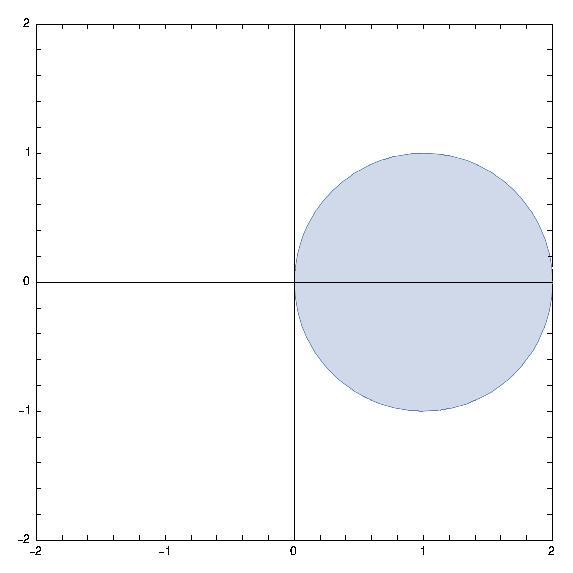
\includegraphics[width=\columnwidth]{stabbdf1e1.eps}\\$\alpha = 1$}%
\only<3>{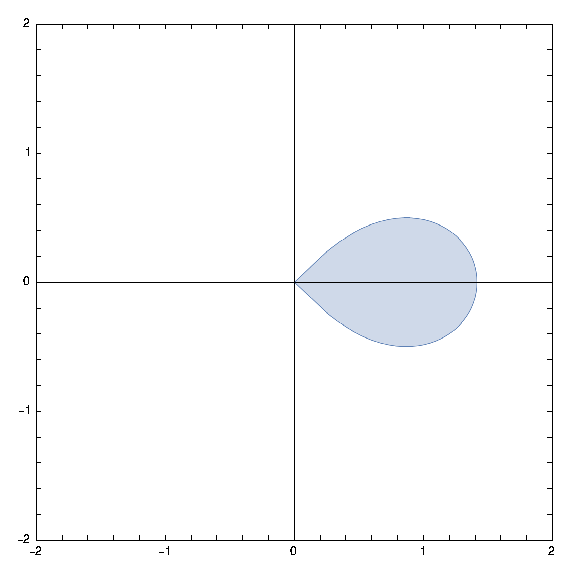
\includegraphics[width=\columnwidth]{stabbdf1e05.eps}\\$\alpha = 0.5$}%
\only<4>{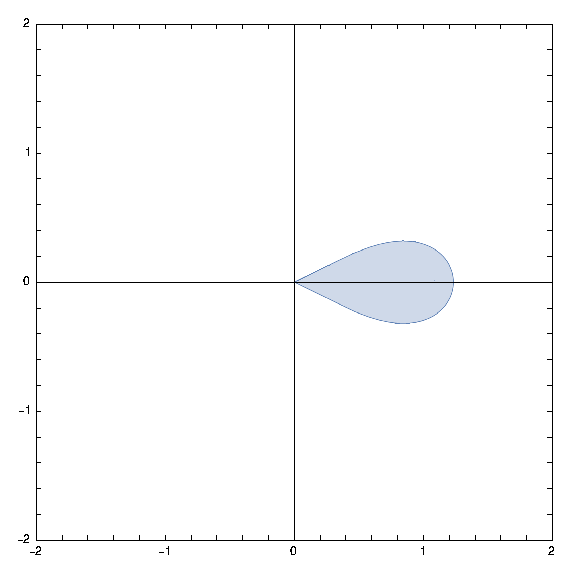
\includegraphics[width=\columnwidth]{stabbdf1e03.eps}\\$\alpha = 0.3$}%
\only<5>{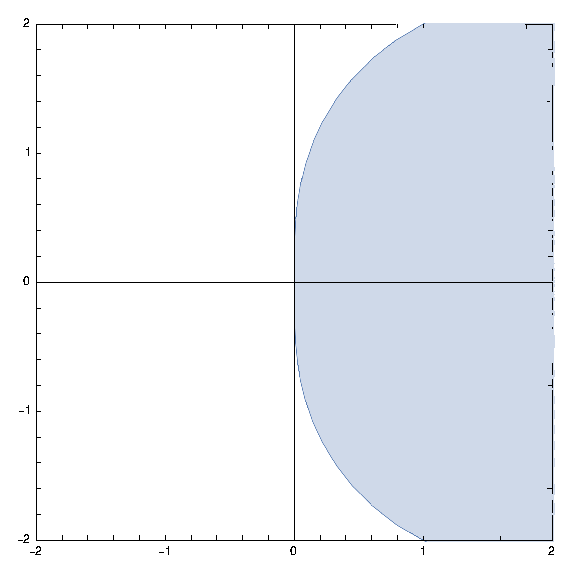
\includegraphics[width=\columnwidth]{stabbdf2e1.eps}\\$\alpha = 1$}%
\only<6>{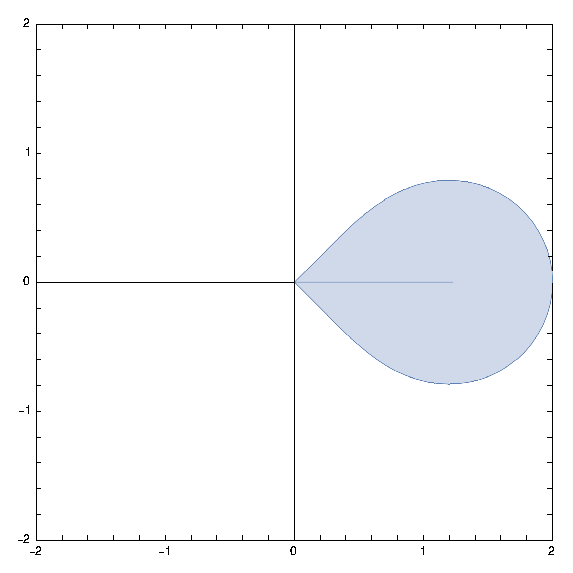
\includegraphics[width=\columnwidth]{stabbdf2e05.eps}\\$\alpha = 0.5$}%
\only<7>{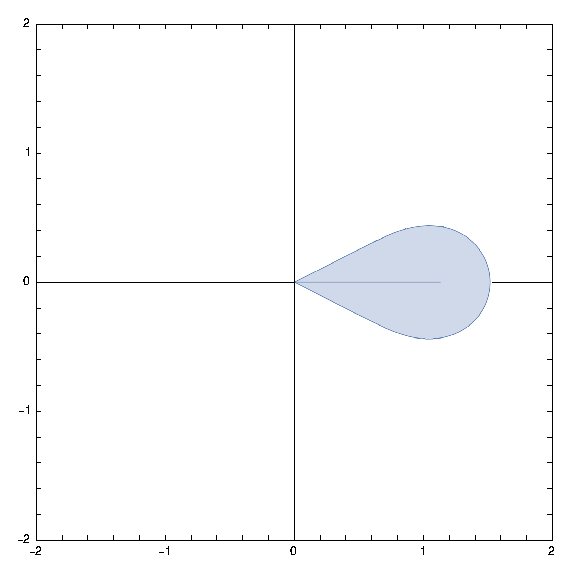
\includegraphics[width=\columnwidth]{stabbdf2e03.eps}\\$\alpha = 0.3$}%
\begin{onlyenv}<8>
\begin{block}{\faQuestionCircle\, How do we obtain the coefficients?}
How can we obtain the coefficient describing the method?
\end{block}
\end{onlyenv}
\end{column}
\end{columns}
\vfill

\only<2-4>{For $p = 1$ we can consider the stability region $S = \mathbb{C} \setminus \left\lbrace \nicefrac{1}{\omega(\zeta)} \,:\; |\zeta| \leq 1 \right\rbrace$ and plot the part of the $\mathbb{C}$-plane we have to remove.}
\only<5-7>{For $p = 1$ we can consider the stability region $S = \mathbb{C} \setminus \left\lbrace \nicefrac{1}{\omega(\zeta)} \,:\; |\zeta| \leq 1 \right\rbrace$ and plot the part of the $\mathbb{C}$-plane we have to remove.}

\end{frame}

\begin{frame}{Computing the FLMM coefficients}

We have now the converse of the previous problem, we have a closed expression for $\omega(\zeta)$, and now we need the coefficients to write
\[
I_\tau^\alpha g(t_n) = \tau^\alpha \sum_{j=0}^{n} \omega_{n-j} g(t_j) + \tau^\beta \sum_{j=0}^{s} w_{n,j} g(t_j),
\]
\begin{itemize}
	\item $\{\omega_{j}\}_{j=0}^n$ convolution coefficients from $\omega(\zeta)$,
	\item $\{w_{n,j}\}_{j=0}^{k}$ starting quadrature weights. 
\end{itemize}

\begin{itemize}
	\item<2-> For the convolution coefficients we can use:
	\begin{itemize}
		\item<3->[\faDoorClosed] Fast Fourier Transform (FFT) techniques for formal power series,
		\item<4->[\faDoorClosed] A recursion technique for complex binomial series. 
	\end{itemize}
	\item<5-> Solving a small $k \times k$ Vandermonde system. 
\end{itemize}

\end{frame}

\begin{frame}{The Newton Method for Power Series~\parencite{HenriciFFTMethods}}

Let us suppose that $\alpha = \nicefrac{1}{2}$ and that we have a power series of the form
\[
\omega(\zeta) = \sum_{j=0}^{+\infty} \omega_j \zeta^j,
\]
for which we want to compute for a generic $p$th degree BDF
\only<1>{
\[
\omega(\zeta)^{-2} = q(\zeta) \text{ with } q(\zeta) = \sum_{k=1}^{p} \frac{1}{k}(1-\zeta)^k,
\]
}\only<2>{
\[
F(\omega(\zeta)) = 0 \text{ with } F(w) = w^{-2} - q(\zeta).
\]
}

\only<3>{
To which we can apply the Newton's method for power series
\[
\begin{cases}
\omega^{(0)}(\zeta) = \omega_0, \\
\omega^{(m+1)}(\zeta) = \left[ \omega^{(m)}(\zeta) - F'(\omega^{(m)}(\zeta))^{-1} F(\omega^{(m)}(\zeta)) \right]_{2^{m+1}},
\end{cases}
\]
for $[ \cdot ]_k$ the truncation operator for a power series, i.e., $\left[ \sum_{j=0}^{+\infty} a_j \zeta^j \right]_k = \sum_{j=0}^{k} a_j \zeta^j$, and $\omega_0$ the solution of $[F(\omega_0)]_1 = 0$.	
}
\only<4>{
To which we can apply the Newton's method for power series
\[
\begin{cases}
\omega^{(0)}(\zeta) = \omega_0 = q(0)^{-\nicefrac{1}{2}}, \\
\omega^{(m+1)}(\zeta) = \left[ \nicefrac{3}{2} \omega^{(m)}(\zeta) - \nicefrac{1}{2}\left(\omega^{(m)}(\zeta)\right)^3 q(\zeta) \right]_{2^{m+1}},
\end{cases}
\]
for $[ \cdot ]_k$ the truncation operator for a power series, i.e., $\left[ \sum_{j=0}^{+\infty} a_j \zeta^j \right]_k = \sum_{j=0}^{k} a_j \zeta^j$.

After $m$ step we have that
\[
\omega^{(m)}(\zeta) = [\omega(\zeta)]_{2^m} = \sum_{j=0}^{2^m-1} \omega_j \zeta^j \quad \forall m \geq 0\, \text{ and cost } O(2^m \log(2^m)).
\]
}
\end{frame}

\begin{frame}{Recurrence relation}

\begin{alertblock}{Theorem~\cite[Theorem 1.6c, p. 42]{HenriciBook}}
Let $\phi(\zeta) = 1 + \sum_{n=1}^{+\infty} a_n \zeta^n$ be a formal power series. Then for any $\alpha \in \mathcal{C}$, we have
\[
(\phi(\zeta))^\alpha = \sum_{n=0}^{+\infty} v_n^{(\alpha)} \zeta^n,
\]
where coefficients $v_n^{(\alpha)}$ can be evaluated recursively as
\[
 v_0^{(\alpha)} = 1, \qquad v_n^{(\alpha)} = \sum_{j=1}^{n} \left( \frac{(\alpha +1)j}{n} - 1 \right) a_j v_{n-j}^{(\alpha)}
\]
\end{alertblock}

\begin{itemize}
	\item[\faMoneyBillWave] This approach costs an $O(N^2)$ in general, but can be simplified, e.g., when $a_1 = \pm 1$, and $a_i > 0$ for $i > 1$ it involves only $2N$ multiplications and $N$ additions.
\end{itemize}

\end{frame}

\begin{frame}{Computing the starting weights}
The starting weights $w_{n,j}$ in 
\[
I_\tau^\alpha g(t_n) = \tau^\alpha \sum_{j=0}^{n} \omega_{n-j} g(t_j) + \tau^\beta \sum_{j=0}^{s} w_{n,j} g(t_j),
\]
are introduced to deal with the singular behavior of the solution close to the left endpoint of the integration interval.

\begin{block}<2->{Starting weight selection}
We fix them by imposing that $I_\tau^\alpha t^\nu$ is exact for $\nu \in \mathcal{A} = \mathcal{A}_{p-1} \cup \{p-1\}$ with $p$ the order of convergence of the FLMM, and  $\mathcal{A}_{p-1} = \{ \nu \in \mathbb{R} \,|\; \nu = i + j \alpha, \quad i,j \in \mathbb{N}, \nu < {p-1}\}$.
\end{block}

\onslide<3>{
\[
\tau^\alpha \sum_{j=0}^{s} w_{n,j} (jh)^\nu = \frac{1}{\Gamma(\alpha)} \int_{0}^{n\tau} (n\tau - \xi)^{\alpha-1} \chi^\nu\,\textrm{d}\chi - \tau^\alpha \sum_{j=0}^{n} \omega_{n-j} (jh)^\nu, \quad \nu \in \mathcal{A}. 
\]	
}

\end{frame}

\begin{frame}{Solving the Vandermonde system}
The resulting linear system is of ``real'' Vandermonde type, i.e.,
\[
(A)_{j,\nu_i = 1}^s = (jh)^{\nu_i}, \qquad \nu_{i} \in A, \quad s = |\mathcal{A}|.
\]
\begin{itemize}
	\item The condition number depends on $\alpha$!
	\item<2-> If $\alpha = \nicefrac{1}{M}$ for some integer $M$ then we can rewrite the system in the ``integer'' Vandermonde form, thus \emph{mildly} ill-conditioned,
	\item<3-> If $\alpha = \nicefrac{1}{M} - \epsilon$ and $p \geq 2$, then $\mathcal{A}$ will contain $1$ and $M\alpha = 1 - M\epsilon$, hence the matrix will have two almost identical columns, thus a \emph{bad} ill-conditioning.
	\item<4-> The right-hand side 
	\[
	\frac{1}{\Gamma(\alpha)} \int_{0}^{n\tau} (n\tau - \xi)^{\alpha-1} \chi^\nu\,\textrm{d}\chi - \tau^\alpha \sum_{j=0}^{n} \omega_{n-j} (jh)^\nu
	\]
	can suffer from cancellation of digits!
\end{itemize}

\end{frame}

\begin{frame}{\faCompass\,Where are we?}
\definecolor{success}{HTML}{4a934a}
\definecolor{todo}{HTML}{0099cc}

We know a general way to obtain FLMM methods of the form
\[
y^{(n)} = T_{m-1}(t_n) + \tau^\beta \sum_{j=0}^{s} \alert<3>{w_{n,j}} f(t_j,y^{(j)}) + \tau^\alpha \sum_{j=0}^{n} \alert<2>{\omega_{n-j}} f(t_j,y^{(j)}),
\]
\begin{itemize}
	\item[\textcolor{success}{\faCheckCircle}]<1-> starting from the polynomials $(\rho,\sigma)$ of an implicit order $p$ method,
	\item[\textcolor{success}{\faCheckCircle}]<2-> we have seen how to compute the convolution coefficients $\omega_n$,
	\item[\textcolor{success}{\faCheckCircle}]<3-> we have seen how to compute the starting nodes $w_{n,j}$,
	\item[\textcolor{todo}{\faClipboardList}]<4-> we need to discuss how we compute the starting values for a multi-step method,
	\item[\textcolor{todo}{\faClipboardList}]<5-> we still need to discuss how we can efficiently treat the memory term.
\end{itemize}

\end{frame}
%
%\begin{frame}{Computing the starting values}\small
%To initialize the computation we need the values $y^{(0)},\ldots,y^{(s)}$, $s+1$, $s = |\mathcal{A}|$. 
%\begin{itemize}
%	\item<2-> We know $y^{(0)}$ from the initial condition, thus we have to solve for the remaining ones.
%	\item<3-> To avoid mixing methods we evaluate all the approximations at the same time by solving
%	\[
%	\begin{bmatrix}
%	y^{(1)}\\
%	y^{(2)}\\
%	\vdots\\
%	y^{(s)}
%	\end{bmatrix} = \begin{bmatrix}
%	T_{m-1}(t_1) \\
%	T_{m-1}(t_2) \\
%	\vdots \\
%	T_{m-1}(t_s) \\
%	\end{bmatrix}
%	+ \tau^\alpha \begin{bmatrix}
%	(\omega_1 + w_{1,0}) f_0 \\
%	(\omega_2 + w_{2,0}) f_0 \\
%	\vdots \\
%	(\omega_s + w_{s,0}) f_0 
%	\end{bmatrix}
%	+ \tau^\alpha \left( \Omega \otimes I + W \otimes I \right) \begin{bmatrix}
%	f(t_1,y^{(1)}) \\
%	f(t_2,y^{(2)}) \\
%	\vdots \\
%	f(t_s,y^{(s)}) \\
%	\end{bmatrix}  
%	\]
%	\only<3>{where
%	\[
%	\Omega = \begin{bmatrix}
%	\omega_0 & \\
%	\omega_1 & \omega_0 \\
%	\vdots & \vdots & \ddots \\
%	\omega_{s-1} & \omega_{s-2} & \cdots & \omega_0 
%	\end{bmatrix}, \quad W = \begin{bmatrix}
%	w_{1,1} & w_{1,2} & \cdots & w_{1,s} \\
%	w_{2,1} & w_{2,2} & \cdots & w_{2,s} \\
%	\vdots & \vdots & \ddots & \vdots \\
%	w_{s,1} & w_{s,2} & \cdots & w_{s,s} 
%	\end{bmatrix}
%	\]}
%\only<4->{
%	\item<4-> This will be in general an $s \times \dim(y^{(j)})$ nonlinear system that we need to solve before starting the iteration.
%	\item<5-> If the value of $\alpha$ is not very small, viz $s$ is moderate, and the system of ODEs is moderate this is manageable. 
%}
%\end{itemize}
%\end{frame}
%
%\begin{frame}{Treating the memory term}
%If we compute the sum on the coefficients $\omega_{j}$ naively for
%\[
%y^{(n)} = T_{m-1}(t_n) + \tau^\beta \sum_{j=0}^{s} w_{n,j} f(t_j,y^{(j)}) + \tau^\alpha \alert{\sum_{j=0}^{n} \omega_{n-j} f(t_j,y^{(j)})},
%\]
%we end up having a $O(N^2)$ cost! If we do not perform this task efficiently the numerical solution degenerates in an unworkable task as we either refine our
%grid or enlarge our computational domain.
%
%\begin{itemize}
%	\item[\faDoorClosed]<2-> We can try to ``forget'' part of the lag-term,
%	\item[\faDoorClosed]<3-> We can consider using a stretched grid towards $t_0$ to reduce $N$,
%	\item[\faDoorClosed]<4-> We can try an approach with nested meshes to reduce the load,
%	\item[\faDoorClosed]<5-> We can exploit the fact that this is a convolution and adopt some FFT tricks.
%\end{itemize}
%
%\end{frame}
%
%\begin{frame}{The FFT trick~\parencite{HairerFFTtrick}}
%
%The treatment remains the same indifferently for both PI and FLMM method, let us focus here on the generic formulation
%\[
%y^{(n)} = \phi_n + \sum_{j=0}^{n} c_{n-j} f_j.
%\]
%
%\begin{itemize}
%	\item<2-> Let $r$ be a moderate number of step, e.g., $r = 2^k$ for a small $k$, we compute the first step directly
%	\[
%	y^{(n)} = \phi_n + \sum_{j=0}^{n} c_{n-j} f_j, \quad n = 0,1,\ldots,r-1.
%	\]
%	\item<3-> If we now want to compute the next $r$ approximations we can separate the lag term as
%	\[
%	y^{(n)} = \phi_n + \sum_{j=0}^{r-1} c_{n-j} f_j + \sum_{j=r}^{n} c_{n-j} f_j, \quad n \in \{r,r+1,\ldots,2r-1\}.
%	\]
%\end{itemize}
%\end{frame}
%
%\begin{frame}{The FFT trick~\parencite{HairerFFTtrick}}
%\only<1-3>{
%\begin{itemize}
%	\item<1-> If we now want to compute the next $r$ approximations we can separate the lag term as
%\[
%y^{(n)} = \phi_n + \sum_{j=0}^{r-1} c_{n-j} f_j + \sum_{j=r}^{n} c_{n-j} f_j, \quad n \in \{r,r+1,\ldots,2r-1\}.
%\]
%\end{itemize}}
%\begin{onlyenv}<2>
%	\begin{exampleblock}{\faLightbulb\,We can use FFT!}
%		If we call $S_r(n,0,r-1) = \sum_{j=0}^{r-1} c_{n-j}f_j$, $n \in \{r,r+1,\ldots,2r-1\}$, the set of partial sums each of length $r$ we can evaluate them with FFT in $O(2r \log_2(2r))$.
%	\end{exampleblock}
%\end{onlyenv}
%\begin{onlyenv}<4>
%	\begin{exampleblock}{\faLightbulb\,We can use FFT!}
%		If we call $S_{2r}(n,0,2r-1) = \sum_{j=0}^{2r-1} c_{n-j}f_j$, and $S_{r}(n,2r,3r-1) = \sum_{j=2r}^{3r-1} c_{n-j}f_j$ the set of partial sums of lengths $2r$ and $r$ we can evaluate them with FFT in $O(4r \log_2(4r))$ and $O(2r \log_2(2r))$ respectively.
%	\end{exampleblock}
%\end{onlyenv}
%\begin{onlyenv}<3->
%\begin{itemize}
%	\item<3-> We can apply the same process recursively if we double every time-interval under consideration
%	\[
%	\begin{split}
%	y^{(n)} = & \phi_n + \sum_{j=0}^{2r-1} c_{n-j} f_j + \sum_{j=2r}^{n} c_{n-j} f_j, \quad n \in \{2r,2r+1,\ldots,3r-1\}, \\
%	y^{(n)} = & \phi_n + \sum_{j=0}^{2r-1} c_{n-j} f_j + \sum_{j=2r}^{3r-1} c_{n-j} f_j + \sum_{j=3r}^{n} c_{n-j} f_j, \quad n \in \{3r,3r+1,\ldots,4r-1\},
%	\end{split}
%	\]
%	
%\end{itemize}
%\end{onlyenv}
%\end{frame}
%
%\begin{frame}[fragile]{The FFT trick~\parencite{HairerFFTtrick}}
%\begin{columns}
%\begin{column}{0.45\columnwidth}\only<1-9>{
%\definecolor{qqqqww}{rgb}{0,0,0.4}
%\definecolor{ffzzqq}{rgb}{1,0.6,0}
%\definecolor{fftttt}{rgb}{1,0.2,0.2}
%\definecolor{zzzzff}{rgb}{0.6,0.6,1}
%\begin{tikzpicture}[line cap=round,line join=round,>=triangle 45,x=0.35cm,y=0.35cm]
%\clip(-0.6,-0.6) rectangle (16.3,16.3);
%\fill[color=zzzzff,fill=zzzzff,fill opacity=0.1] (2,0) -- (4,0) -- (4,2) -- (2,2) -- cycle;
%\fill[color=fftttt,fill=fftttt,fill opacity=0.1] (4,0) -- (8,0) -- (8,4) -- (4,4) -- cycle;
%\fill[color=ffzzqq,fill=ffzzqq,fill opacity=0.1] (8,0) -- (16,0) -- (16,8) -- (8,8) -- cycle;
%\fill[color=zzzzff,fill=zzzzff,fill opacity=0.1] (6,4) -- (8,4) -- (8,6) -- (6,6) -- cycle;
%\fill[color=zzzzff,fill=zzzzff,fill opacity=0.1] (10,8) -- (12,8) -- (12,10) -- (10,10) -- cycle;
%\fill[color=fftttt,fill=fftttt,fill opacity=0.1] (12,8) -- (16,8) -- (16,12) -- (12,12) -- cycle;
%\fill[color=zzzzff,fill=zzzzff,fill opacity=0.1] (14,12) -- (16,12) -- (16,14) -- (14,14) -- cycle;
%\fill[color=qqqqww,fill=qqqqww,fill opacity=0.1] (4,4) -- (6,4) -- (5.99,5.99) -- cycle;
%\fill[color=qqqqww,fill=qqqqww,fill opacity=0.1] (5.99,5.99) -- (8,6) -- (8,8) -- cycle;
%\fill[color=qqqqww,fill=qqqqww,fill opacity=0.1] (8,8) -- (10,8) -- (10,10) -- cycle;
%\fill[color=qqqqww,fill=qqqqww,fill opacity=0.1] (10,10) -- (12,10) -- (12,12) -- cycle;
%\fill[color=qqqqww,fill=qqqqww,fill opacity=0.1] (12,12) -- (14,12) -- (14,14) -- cycle;
%\fill[color=qqqqww,fill=qqqqww,fill opacity=0.1] (14,14) -- (16,14) -- (16,16) -- cycle;
%\fill[color=qqqqww,fill=qqqqww,fill opacity=0.1] (0,0) -- (2,0) -- (1.99,1.99) -- cycle;
%\fill[color=qqqqww,fill=qqqqww,fill opacity=0.1] (1.99,1.99) -- (4,2) -- (4,4) -- cycle;
%\draw (0,0)-- (16,16);
%\draw (16,16)-- (16,0);
%\draw (16,0)-- (0,0);
%\draw [color=zzzzff] (2,0)-- (4,0);
%\draw [color=zzzzff] (4,0)-- (4,2);
%\draw [color=zzzzff] (4,2)-- (2,2);
%\draw [color=zzzzff] (2,2)-- (2,0);
%\draw [color=fftttt] (4,0)-- (8,0);
%\draw [color=fftttt] (8,0)-- (8,4);
%\draw [color=fftttt] (8,4)-- (4,4);
%\draw [color=fftttt] (4,4)-- (4,0);
%\draw [color=ffzzqq] (8,0)-- (16,0);
%\draw [color=ffzzqq] (16,0)-- (16,8);
%\draw [color=ffzzqq] (16,8)-- (8,8);
%\draw [color=ffzzqq] (8,8)-- (8,0);
%\draw [color=zzzzff] (6,4)-- (8,4);
%\draw [color=zzzzff] (8,4)-- (8,6);
%\draw [color=zzzzff] (8,6)-- (6,6);
%\draw [color=zzzzff] (6,6)-- (6,4);
%\draw [color=zzzzff] (10,8)-- (12,8);
%\draw [color=zzzzff] (12,8)-- (12,10);
%\draw [color=zzzzff] (12,10)-- (10,10);
%\draw [color=zzzzff] (10,10)-- (10,8);
%\draw [color=fftttt] (12,8)-- (16,8);
%\draw [color=fftttt] (16,8)-- (16,12);
%\draw [color=fftttt] (16,12)-- (12,12);
%\draw [color=fftttt] (12,12)-- (12,8);
%\draw [color=zzzzff] (14,12)-- (16,12);
%\draw [color=zzzzff] (16,12)-- (16,14);
%\draw [color=zzzzff] (16,14)-- (14,14);
%\draw [color=zzzzff] (14,14)-- (14,12);
%\draw [color=qqqqww] (4,4)-- (6,4);
%\draw [color=qqqqww] (6,4)-- (5.99,5.99);
%\draw [color=qqqqww] (5.99,5.99)-- (4,4);
%\draw [color=qqqqww] (5.99,5.99)-- (8,6);
%\draw [color=qqqqww] (8,6)-- (8,8);
%\draw [color=qqqqww] (8,8)-- (5.99,5.99);
%\draw [color=qqqqww] (8,8)-- (10,8);
%\draw [color=qqqqww] (10,8)-- (10,10);
%\draw [color=qqqqww] (10,10)-- (8,8);
%\draw [color=qqqqww] (10,10)-- (12,10);
%\draw [color=qqqqww] (12,10)-- (12,12);
%\draw [color=qqqqww] (12,12)-- (10,10);
%\draw [color=qqqqww] (12,12)-- (14,12);
%\draw [color=qqqqww] (14,12)-- (14,14);
%\draw [color=qqqqww] (14,14)-- (12,12);
%\draw [color=qqqqww] (14,14)-- (16,14);
%\draw [color=qqqqww] (16,14)-- (16,16);
%\draw [color=qqqqww] (16,16)-- (14,14);
%\draw [color=qqqqww] (0,0)-- (2,0);
%\draw [color=qqqqww] (2,0)-- (1.99,1.99);
%\draw [color=qqqqww] (1.99,1.99)-- (0,0);
%\draw [color=qqqqww] (1.99,1.99)-- (4,2);
%\draw [color=qqqqww] (4,2)-- (4,4);
%\draw [color=qqqqww] (4,4)-- (1.99,1.99);
%\begin{scriptsize}
%\fill [color=black] (0,0) circle (1.5pt);
%\draw[color=black] (-0.06,-0.24) node {0};
%\fill [color=black] (2,0) circle (1.5pt);
%\draw[color=black] (1.98,-0.24) node {r};
%\fill [color=black] (4,0) circle (1.5pt);
%\draw[color=black] (3.61,-0.26) node {2r};
%\fill [color=black] (8,0) circle (1.5pt);
%\draw[color=black] (7.9,-0.13) node {4r};
%\fill [color=black] (16,0) circle (1.5pt);
%\draw[color=black] (15.81,-0.11) node {8r};
%\draw[color=zzzzff] (3.17,1.16) node {$S_r$};
%\draw[color=fftttt] (6.42,2.16) node {$S_{2r}$};
%\draw[color=ffzzqq] (12.43,4.16) node {$S_{4r}$};
%\draw[color=zzzzff] (7.17,5.16) node {$S_r$};
%\draw[color=zzzzff] (11.19,9.15) node {$S_r$};
%\draw[color=fftttt] (14.43,10.15) node {$S_{2r}$};
%\draw[color=zzzzff] (15.18,13.15) node {$S_r$};
%\draw[color=qqqqww] (5.5,4.82) node {$T_r$};
%\draw[color=qqqqww] (7.5,6.82) node {$T_r$};
%\draw[color=qqqqww] (9.52,8.82) node {$T_r$};
%\draw[color=qqqqww] (11.52,10.82) node {$T_r$};
%\draw[color=qqqqww] (13.52,12.82) node {$T_r$};
%\draw[color=qqqqww] (15.52,14.82) node {$T_r$};
%\draw[color=qqqqww] (1.5,0.82) node {$T_r$};
%\draw[color=qqqqww] (3.5,2.82) node {$T_r$};
%\end{scriptsize}
%\end{tikzpicture}}%
%\only<10>{
%% This file was created by matlab2tikz.
%
%The latest updates can be retrieved from
%  http://www.mathworks.com/matlabcentral/fileexchange/22022-matlab2tikz-matlab2tikz
%where you can also make suggestions and rate matlab2tikz.
%
\begin{center}
\definecolor{mycolor1}{rgb}{0.00000,0.44700,0.74100}%
\definecolor{mycolor2}{rgb}{0.85000,0.32500,0.09800}%
%
\begin{tikzpicture}

\begin{axis}[%
width=0.8\columnwidth,
height=0.75\columnwidth,
at={(1.142in,0.473in)},
scale only axis,
xmode=log,
xmin=1,
xmax=100000,
xminorticks=true,
xlabel style={font=\color{white!15!black}},
xlabel={N},
ymode=log,
ymin=10,
ymax=1000000000,
yminorticks=true,
axis background/.style={fill=white},
xmajorgrids,
xminorgrids,
ymajorgrids,
yminorgrids,
legend style={at={(0.03,0.97)}, anchor=north west, legend cell align=left, align=left, draw=white!15!black}
]
\addplot [color=mycolor1, line width=2.0pt, mark=o, mark options={solid, mycolor1}]
  table[row sep=crcr]{%
4	16\\
8	64\\
16	256\\
32	1024\\
64	4096\\
128	16384\\
256	65536\\
512	262144\\
1024	1048576\\
2048	4194304\\
4096	16777216\\
8192	67108864\\
16384	268435456\\
};
\addlegendentry{$\text{N}^\text{2}$}

\addplot [color=mycolor2, dashed, line width=2.0pt, mark=x, mark options={solid, mycolor2}]
  table[row sep=crcr]{%
4	16\\
8	72\\
16	256\\
32	800\\
64	2304\\
128	6272\\
256	16384\\
512	41472\\
1024	102400\\
2048	247808\\
4096	589824\\
8192	1384448\\
16384	3211264\\
};
\addlegendentry{$\text{N log}_\text{2}\text{(N)}^\text{2}$}

\end{axis}
\end{tikzpicture}%
\end{center}
%}
%\end{column}
%\begin{column}{0.55\columnwidth}%
%\definecolor{qqqqww}{rgb}{0,0,0.4}%
%\definecolor{ffzzqq}{rgb}{1,0.6,0}%
%\definecolor{fftttt}{rgb}{1,0.2,0.2}%
%\definecolor{zzzzff}{rgb}{0.6,0.6,1}%
%\only<1-2>{
%\begin{itemize}
%	\item We can iterate the process for the $4r$ approximations in the interval $n \in \{ 4r,\ldots,8r-1\}$, together
%	with the partial sums $S_{4r}(n,0,4r-1)$, $S_{2r}(n,4r,6r-1)$, $S_{r}(n,6r,7r-1)$ that can be evaluated in
%	$O(8r \log_2(8r))$, $O(4r \log_2(4r))$ and $O(2r \log_2(2r))$ respectively,
%	\item<2-> At each level we have to complete the recursion by computing\vspace{-1em}
%	\[
%	\begin{split}
%	T_r(p,n) = & \sum_{j=p}^{n} c_{n-j} f_j, \; p = \ell r, \\ n \in & \{\ell r, \ell r + 1,\ldots,(\ell+1)r-1\}, \\ \ell = & 0,1,2,\ldots.
%	\end{split}
%	\]
%\end{itemize}}%
%\only<3->{
%To determine the whole cost we just have to sum the various components
%\begin{itemize}
%	\item<4-> Assume that $N = 2^{n_t}$
%	\item<5-> $O(N \log_2 N)$ for \textcolor{ffzzqq}{$S_{4r}$},
%	\item[$+$]<6-> $O( \nicefrac{N}{2} \log_2 \nicefrac{N}{2})$ for $2$ \textcolor{fftttt}{$S_{2r}$}
%	\item[$+$]<7-> $O( \nicefrac{N}{4} \log_2 \nicefrac{N}{4})$ for $4$ \textcolor{zzzzff}{$S_r$}
%	\item[$+$]<8-> $\nicefrac{r(r+1)}{2}$ for the $N/r$ convolutions \textcolor{qqqqww}{$T_r$}
%	\item<9-> In general:
%\only<9>{\[
%	\begin{split}
%	N \log_2 N + 2 \frac{N}{2} \log_2 \frac{N}{2} + 4 \frac{N}{4}\log_2 \frac{N}{4} + \cdots \\ + p \frac{N}{p} \log_2 \frac{N}{p} + \frac{N}{r} \frac{r(r+1)}{2}, \quad p = \frac{N}{2r} 
%	\end{split}
%	\]}
%\only<10>{
%\[
%\begin{split}
%\sum_{j=0}^{\log_2 p} N \log_2 \frac{N}{2^j} + N \frac{r+1}{2} = O(N (\log_2 N)^2 ).
%\end{split}
%\]
%}
%\end{itemize}
%}
%\end{column}
%\end{columns}
%\end{frame}
%
%\begin{frame}{Short-memory principle~\parencite{FordSpeedAccuracy}}
%We can try to use a ``fixed memory length'' to reduce the computational (and memory) load.
%\[
%\begin{split}
%y(t_{n+1}) =  y(t_n) & + \frac{1}{\Gamma(\alpha)} \int_{t_n}^{t_{n+1}} (t_{n+1}-\tau)^{\alpha-1} f(\tau,x(\tau))\,\textrm{d}\tau \\
%& + \frac{1}{\Gamma(\alpha)} \int_{0}^{t_n} ( (t_{n+1} - \tau)^{\alpha-1} - (t_n - \tau)^{\alpha-1} ) f(\tau,y(\tau))\,\textrm{d}\tau, \quad \alpha \in (0,1).
%\end{split} 
%\]
%\only<2->{Let us introduce now a fixed window $T_M$ of memory, then}
%\only<2-7>{
%\[
%\begin{split}
%E = & \left| \frac{1}{\Gamma(\alpha)} \int_{0}^{t_n - T_M} ( (t_{n+1} - \tau)^{\alpha-1} - (t_n - \tau)^{\alpha-1} ) f(\tau,y(\tau))\,\textrm{d}\tau \right| \\ \leq &  \frac{M}{\Gamma(\alpha)} \left| \int_{0}^{t_n - T_M} ( (t_{n+1} - \tau)^{\alpha-1} - (t_n - \tau)^{\alpha-1} )\,\textrm{d}\tau \right|\only<3>{\\
%= & \frac{M}{\alpha \Gamma(\alpha)} \left| (\tau + T_M)^\alpha - t_{n+1}^{\alpha} - T^\alpha + t_n^\alpha \right| }\only<4-5>{\\
%= & \frac{M}{\Gamma(\alpha)} \left| \int_{T_M}^{T_M + \tau} z^{\alpha-1}\,\textrm{d}z - \int_{t_n}^{t_{n+1}} z^{\alpha-1}\,\textrm{d}z \right| \only<5>{ (Mean Value Theorem) } }\only<6>{ \\
%= & \frac{M}{\Gamma(\alpha)} \left| (z_1^*)^{\alpha-1} \tau - (z_2^*)^{\alpha-1} \tau \right| \quad z_1^* \in [T_M,T_M+\tau], \; z_2^* \in [t_n,t_{n+1}]
%}\only<7>{ \\
%< & \frac{M}{\Gamma(\alpha)} T_M^{\alpha-1} \tau, \qquad \alpha \in (0,1).
%}
%\end{split}
%\]
%}\only<8>{
%\[
%E = \left| \frac{1}{\Gamma(\alpha)} \int_{0}^{t_n - T_M} ( (t_{n+1} - \tau)^{\alpha-1} - (t_n - \tau)^{\alpha-1} ) f(\tau,y(\tau))\,\textrm{d}\tau \right|  < \frac{M}{\Gamma(\alpha)} T_M^{\alpha-1} \tau, \quad \alpha \in (0,1).
%\]
%}\only<9>{
%If we have a global error bound $E_{\text{global}}$ with step-length $\tau$ we just need to choose
%\[
%T_M > \left( \frac{M}{\Gamma(\alpha)E_{\text{global}}} \right)^{\nicefrac{1}{1-\alpha}}, \quad \alpha \in (0,1),
%\] 
%while if we have a local error bound $E_{\text{local}}$
%\[
%T_M > \left( \frac{M\tau}{\Gamma(\alpha)E_{\text{local}}} \right)^{\nicefrac{1}{1-\alpha}}, \quad \alpha \in (0,1).
%\]
%}
%\end{frame}
%
%\begin{frame}{Short-memory principle~\parencite{FordSpeedAccuracy}}
%
%\begin{itemize}
%	\item[\faSmile]<1-> In case $\alpha \in (0,1)$ the short memory method with fixed length can be effective and the length T is independent of the full
%	interval of integration.
%	\item[\faSadTear]<2-> Similar bounds can be written for the case $\alpha > 1$, that is
%	\[
%	E < \frac{M}{\Gamma(\alpha)} (t_{n+1}^\alpha - T_M^{\alpha-1})\tau, \quad \alpha > 1.
%	\]
%	But now to preserve the order of accuracy, we must choose
%	\[
%	T_M^{\alpha - 1} > t_{n+1}^{\alpha-1} - \frac{E_{\text{global}} \Gamma(\alpha)}{M}, \quad \alpha > 1,
%	\]
%	that we will make us lose all the computational gain.
%\end{itemize}
%
%\onslide<3>{The idea can be refined by using \emph{nested meshes}.}
%
%\end{frame}
%
%\begin{frame}{Nested meshes}
%Zeroing out the memory term is too drastic, we may want to relax this.
%
%\begin{exampleblock}<2->{Scaling properties}
%\only<2>{\[I^{\alpha}_{[0,t]} 
%	f(t) = \int_{0}^{t} 
%	\frac{f(\tau)}{(t-\tau)^{1-\alpha}}\,\textrm{d}\tau\]}
%\only<3>{\[
%	I^{\alpha}_{[0,t]} f(w t) = \int_{0}^{t} \frac{f(\tau)}{(wt-\tau)^{1-\alpha}}\,\textrm{d}\tau\]}
%\only<4>{\[
%	I^{\alpha}_{[0,t]} f(w t) = w^\alpha \int_{0}^{t} \frac{f(w\tau)}{(t-\tau)^{1-\alpha}}\,\textrm{d}\tau\]}
%\only<5->{
%	Given $p \in \mathbb{N}$ we then have
%	\[
%	I^{\alpha}_{[0,t]} f(w^p t) = w^{p\alpha} \int_{0}^{t} \frac{f(w^p \tau)}{(t-\tau)^{1-\alpha}}\,\textrm{d}\tau\]
%}
%\end{exampleblock}
%\begin{itemize}
%	\item[\faLightbulb]<6-> We can use the weight on the mesh \[\Omega_\tau^\alpha f(n\tau) \approx I^{\alpha}_{[0,t]} f(n\tau), \text{ step length }\tau\] to compute
%	\[
%	\Omega^\alpha_{w^p \tau} f(w^p n \tau) \approx I^{\alpha}_{[0,t]} f(nw^p\tau), \text{ step length } w^p \tau
%	\]
%	\item<7-> In summary for any $p \in \mathbb{N}$ we get\vspace{-0.5em}
%	\[
%	\Omega_\tau^{\alpha} f(n\tau) = \sum_{j=0}^n \omega_{n-j} f(j\tau) \;\Leftrightarrow\; \Omega^\alpha_{w^p \tau} f(n w^p \tau) = w^{p\alpha} \sum_{j=0}^n \omega_{n-j} f(j w^p \tau).
%	\]
%\end{itemize}
%
%\end{frame}
%
%\begin{frame}{Nested meshes~\parencite{FordSpeedAccuracy}}
%\begin{block}{Nested mesh}
%Given $\tau \in \mathbb{R}^+$, the mesh $M_\tau = \{ \tau n, \; n \in \mathbb{N} \}$. Selected $w,r,p \in \mathbb{N}$, $w > 0$, $r > p$, we have $M_{w^p \tau} \supset M_{w^r \tau}$ and we decompose the interval as
%\[
%[0,t] = [0,t-w^m T] \cup [t - w^mT,t-w^{m-1}T] \cup \cdots \cup [t-wT,t-T]\cup[t-T,t]
%\]
%for $m \in \mathbb{N}$ the smallest integer such that $t < w^{m+1} T$.
%\end{block}
%
%\begin{itemize}
%	\item[\faLightbulb]<2-> This links the \textbf{scaling property} with the singularity of the type $1/(t-\tau)^{1-\alpha}$ suggesting that we should distribute the computational effort logarithmically, and not uniformly.
%	\item<3-> We rewrite our integral\only<4>{ using the scaling property} as
%	\[
%	I_{[0,t]}^\alpha f(t) = \only<3>{I_{[t-T,t]}^\alpha f(t) + \sum_{i=0}^{m-1} I_{[t-w^{i+1}T,t-w^iT]}^\alpha f(t) + I_{[0,t-w^mT]}^\alpha f(t)}
%	\only<4>{I_{[t-T,t]}^\alpha f(t) + \sum_{i=0}^{m-1} w^{i\alpha} I_{[t-w T,t-T]}^\alpha f(w^i t) + w^{m\alpha}I_{[0,t-T]}^\alpha f(w^m t).}
%	\]
%\end{itemize}
%
%\end{frame}
%
%\begin{frame}{Nested meshes~\parencite{FordSpeedAccuracy}}
%In the discrete approximation of
%\[
%I_{[0,t]}^\alpha f(t) = I_{[t-T,t]}^\alpha f(t) + \sum_{i=0}^{m-1} w^{i\alpha} I_{[t-w T,t-T]}^\alpha f(w^i t) + w^{m\alpha}I_{[0,t-T]}^\alpha f(w^m t).
%\]
%we approximate\vspace{-0.5em}
%\[
%\Omega_{\tau,[t-w^{i+1} T,t-w^i T]}^\alpha f(t) \approx \Omega_{w^i \tau,[t-w^{i+1} T,t-w^i T]}^\alpha f(t)
%\]
%and substitute\vspace{-0.5em}
%\[
%w^{i\alpha} \Omega_{\tau,[t-w T,t- T]}^\alpha f(t) = \Omega_{w^i \tau,[t-w^{i+1} T,t- w^{i} T]}^\alpha f(t).
%\]
%\begin{alertblock}<2->{Theorem~\parencite[Theorem~1]{FordSpeedAccuracy}}
%The nested mesh scheme preserves the order of the underlying quadrature
%rule on which it is based.
%\end{alertblock}
%\onslide<3>{\small \textbf{Proof.} For integration over a fixed interval $[0,t]$ the choice of $T$ fixes (independent of $h$) the number of subranges over which the integral is evaluated, on each of them we have en error $O(h^p)$.}
%
%\end{frame}
%
%\begin{frame}{Nested meshes~\parencite{FordSpeedAccuracy}}
%
%\begin{itemize}
%	\item<1-> The first benefit is that we evaluate a fixed number of quadrature coefficients and then re-use them on all successive intervals,
%	\item<2->[\faMoneyBillWave] This approach cost $O(w^m)$ with respect to $O(w^{2m})$ of the full method,
%	\item<3->[\faCog] We could use linear extrapolation techniques to improve the results.
%	\item<4->[\faCog] Selecting the various parameter may need a bit of tuning.
%\end{itemize}
%
%\end{frame}
%
%\section{Codes}
%
%\begin{frame}[fragile]{\faCode\;Available codes}
%With respect to the ordinary case for which there exists many reliable and high-performance codes, the choices for computing the solution of fractional differential equation is much more \emph{sparse}.
%
%\begin{itemize}
%\item From \parencite{garrappa2018numerical}
%\begin{itemize}
%	\item[\faCode] \verb|FDE_PI1_Ex.m| - \href{https://www.dm.uniba.it/members/garrappa/software_folder/fde_pi1_ex.m}{Explicit Product-Integration of rectanguar type}
%	\item[\faCode] \verb|FDE_PI1_Im.m| - \href{https://www.dm.uniba.it/members/garrappa/software_folder/fde_pi1_im.m}{Implicit Product-Integration of rectanguar type}
%	\item[\faCode] \verb|FDE_PI2_Im.m| - \href{https://www.dm.uniba.it/members/garrappa/software_folder/fde_pi2_im.m}{Implicit Product-Integration of trapezoidal type}
%	\item[\faCode] \verb|FDE_PI12_PC.m| - \href{https://www.dm.uniba.it/members/garrappa/software_folder/fde_pi12_pc.m}{Product-Integration with predictor-corrector}
%\end{itemize}
%\item From \parencite{GarrappaTrapezoidal}
%\begin{itemize}
%	\item[\faCode] FLMM2 Matlab code - \href{http://www.mathworks.com/matlabcentral/fileexchange/47081-flmm2}{Three implicit second order Fractional Linear Multistep Methods}.
%\end{itemize}
%
%\begin{block}{\faBinoculars\,A remark}
%All these methods use direct-solver for the Newton method inside them, there is space to make improvement on the solution strategies. Furthermore, a challenge that yet remains: can we find a strategy that combines the convolution features and savings on the memory?
%\end{block}
%
%\end{itemize}
%\end{frame}
%
%\section{Conclusions}
%
%\begin{frame}{Conclusions}
%\definecolor{success}{HTML}{4a934a}
%\definecolor{todo}{HTML}{0099cc}
%
%We know a general way to obtain FLMM methods of the form\vspace{-0.5em}
%\[
%y^{(n)} = T_{m-1}(t_n) + \tau^\beta \sum_{j=0}^{s} {w_{n,j}} f(t_j,y^{(j)}) + \tau^\alpha \sum_{j=0}^{n} {\omega_{n-j}} f(t_j,y^{(j)}),
%\]
%\begin{itemize}
%	\item[\textcolor{success}{\faCheckCircle}] starting from the polynomials $(\rho,\sigma)$ of an implicit order $p$ method,
%	\item[\textcolor{success}{\faCheckCircle}] we have seen how to compute the convolution coefficients $\omega_n$,
%	\item[\textcolor{success}{\faCheckCircle}] we have seen how to compute the starting nodes $w_{n,j}$,
%	\item[\textcolor{success}{\faCheckCircle}] we know how we can compute the starting values for a multi-step method by solving a nonlinear system with Newton,
%	\item[\textcolor{success}{\faCheckCircle}] we have some hints on how we can efficiently treat the memory term.
%\end{itemize}
%
%\begin{block}<2>{\faLuggageCart\,Things we didn't pack\ldots}
%There have been some effort in devising methods of Runge-Kutta type~\parencite{FischerRK}, collocation methods, and exponential type integrators. 
%\end{block}
%
%\end{frame}
%
%%\begin{frame}[fragile]{The FRF first implementation}
%%
%%\begin{columns}
%%\begin{column}{0.6\columnwidth}\definecolor{bg}{rgb}{0.95,0.95,0.95}
%%The code is analogous to the one for the fractional integrals 
%%with Newton-Cotes formulas:
%%\begin{minted}[bgcolor=bg,fontsize=\small,breaklines]{matlab}
%%for i=0:N-1
%%% These are the values b0,b1,...,bN-1 we need 
%%% them for all the computations
%%b(i+1) = ((i+1)^alpha - i^alpha)/alpha; 
%%end
%%y(:,1) = y0;
%%c = (tau^alpha/gamma(alpha));
%%for j=1:N-1
%%fy(:,j) = f(t(j),y(:,j)); % New value of f
%%y(:,j+1) = y(:,1) + c*sum(flipud(b(1:j)).'.*fy(:,1:j));
%%end
%%\end{minted}
%%\end{column}
%%\begin{column}{0.4\columnwidth}
%%\begin{itemize}
%%\item[\faCode]<2-> To build the solution we have to keep in memory either the \textbf{previous solutions} or the \textbf{function evaluations},
%%\item[\faCode]<3-> We have to compute:
%%\[
%%\sum_{j=0}^{n-2} b_{n-j-1}f^{(j)},
%%\]
%%this is a \alert{quadratic cost} with $N$.
%%\item<4-> The $1$-step name is related to the number of initial values to start the computation.
%%\end{itemize}
%%\end{column}
%%\end{columns}
%%
%%\end{frame}
%%
%%\begin{frame}[fragile]{The FRF consistency order}
%%\begin{columns}
%%\begin{column}{0.5\columnwidth}
%%We need to investigate the order of approximation of this method.
%%
%%If we apply it to the case
%%\[
%%{}_{CA}D_{[0,t]}^\alpha y(t) = \lambda y(t), \quad y(0) = 0,
%%\]
%%for $t \in [0,]
%%\end{column}
%%\begin{column}{0.5\columnwidth}
%%\centering
%%
%%% This file was created by matlab2tikz.
%
%The latest updates can be retrieved from
%  http://www.mathworks.com/matlabcentral/fileexchange/22022-matlab2tikz-matlab2tikz
%where you can also make suggestions and rate matlab2tikz.
%
\definecolor{mycolor1}{rgb}{0.00000,0.44700,0.74100}%
\definecolor{mycolor2}{rgb}{0.85000,0.32500,0.09800}%
%
\begin{tikzpicture}

\begin{axis}[%
width=0.6\columnwidth,
height=1.2in,
at={(0.772in,0.481in)},
scale only axis,
xmode=log,
xmin=0.001,
xmax=0.5,
xminorticks=true,
xlabel style={font=\color{white!15!black}},
xlabel={$\tau$},
ymode=log,
ymin=6.40306809290377e-05,
ymax=0.5,
yminorticks=true,
ylabel style={font=\color{white!15!black}},
ylabel={$\|y - y_{true}\|_2/\|y_{true}\|_2$},
axis background/.style={fill=white},
legend style={at={(0.97,0.03)}, anchor=south east, legend cell align=left, align=left, draw=none, fill=none}
]
\addplot [color=mycolor1, line width=2.0pt, mark=o, mark options={solid, mycolor1}]
  table[row sep=crcr]{%
0.5	0.05071550339902\\
0.1	0.00816713156811108\\
0.01	0.000683351712442514\\
0.001	6.40306809290377e-05\\
};
\addlegendentry{Relative Error}

\addplot [color=mycolor2, dashed, line width=2.0pt]
  table[row sep=crcr]{%
0.5	0.5\\
0.1	0.1\\
0.01	0.01\\
0.001	0.001\\
};
\addlegendentry{$\tau$}

\end{axis}
\end{tikzpicture}%
%%	
%%\begin{tabular}{ll}
%%\toprule
%%$\tau$ & Error\\
%%\midrule
%%5.00e-01 & 5.07e-02\\
%%1.00e-01 & 8.17e-03\\
%%1.00e-02 & 6.83e-04\\
%%1.00e-03 & 6.40e-05\\
%%\bottomrule
%%\end{tabular}
%%
%%\end{column}
%%\end{columns}
%%\end{frame}
%%
%%\begin{frame}{The Fractional Trapezoidal Formula}
%%
%%\end{frame}
%%
%%\section{Fractional Linear Multistep Methods}
%%
%%\begin{frame}{Fractional Linear Multistep Methods}
%%To 
%%\end{frame}

\appendix

\section*{Bibliography}
{\unnumbered
	\begin{frame}[allowframebreaks,noframenumbering]{Bibliography}
	\small
	\printbibliography
	
\end{frame}
}

\end{document}